% ---------------------------------------------------------------------
% --- Arquivo principal e os demais serao os dos capitulos.
% --- EXPRESSÕES ENTRE <> DEVERÃO SER COMPLETADAS COM A INFORMAÇÃO ESPECÍFICA DO TRABALHO 
% ---------------------------------------------------------------------

\documentclass[ruledheader]{abnt_UFF}

%---pacotes para hiphenizacao e acentuacao em portugues
\usepackage[utf8]{inputenc}
\usepackage[brazilian]{babel}
%\usepackage[latin1]{inputenc}
\usepackage[T1]{fontenc}
%--- pacote para figuras
\usepackage{epsf}
\usepackage[dvips]{epsfig,graphicx}
%\usepackage{subfigure}
\usepackage{subfig}
\usepackage{cite}
\usepackage{textcomp}
\usepackage{caption}
\usepackage{subcaption}
%--- pacote de simbolos
\usepackage{latexsym}
\usepackage{textcomp}

%--- simbolos matematicos
\usepackage{amsmath}
\usepackage{amssymb}

%--- pacote para gerar pseudo-codigo
\usepackage{algorithm}
\usepackage{algorithmic}
\floatname{algorithm}{Algoritmo}

%--- outros pacotes
\usepackage{url}
\usepackage{longtable}
\usepackage{lscape}
\usepackage{amsthm}
\usepackage{todonotes}
\usepackage{verbatim}
\usepackage{graphicx}


%Tabela Colorida
\usepackage{colortbl}
\usepackage{multicol}
\usepackage{multirow}
\usepackage{rotating}

%\usepackage{ulem}



%--- UML
\usepackage{tikz}
\usetikzlibrary{graphs,graphs.standard,arrows,decorations.pathmorphing,positioning,fit,shapes,calc}
\usepackage{tikz-uml}


\hyphenation{
a-de-qua-da-men-te 
di-men-sio-na-men-to 
re-qui-si-to
}
\usepackage{lscape}
\usepackage{listlang}
\lstset{basicstyle=\small}
\renewcommand{\lstlistingname}{Listagem}



%---------usando tipo de fonte padrao
\renewcommand{\ABNTchapterfont}{\bfseries\fontfamily{cmr}\fontseries{b}\selectfont}
\renewcommand{\ABNTsectionfont}{\bfseries\fontfamily{cmr}}



% --- -----------------------------------------------------------------
% --- Documento Principal.
% --- -----------------------------------------------------------------
% \usepackage[pdftex]{hyperref}
% \hypersetup{colorlinks, sitecolor=black, pdftex}
\begin{document}

% --- -----------------------------------------------------------------
% --- Titulo, abstract, dedicatorias e agradecimentos.
% --- Indice geral, lista de figuras e tabelas.
% --- -----------------------------------------------------------------

% --- -----------------------------------------------------------------
% --- Elementos usados na Capa e na Folha de Rosto.
% --- EXPRESSÕES ENTRE <> DEVERÃO SER COMPLETADAS COM A INFORMAÇÃO ESPECÍFICA DO TRABALHO
% --- E OS SÍMBOLOS <> DEVEM SER RETIRADOS 
% --- -----------------------------------------------------------------
\autor{RAFAEL HEITOR CORREIA DE MELO} % deve ser escrito em maiúsculo

\titulo{Uma Proposta de uso de Dispositivo Háptico \\para Treinamento de Anestesia raquidiana}

\instituicao{UNIVERSIDADE FEDERAL FLUMINENSE}

\orientador{Aura Conci, D.Sc.}

\local{NITERÓI}

\data{2021} % ano da defesa


\comentario{Tese de Doutorado apresentada ao Programa de Pós-Graduação em Computação da \mbox{Universidade} Federal Fluminense como requisito parcial para a obtenção do Grau de \mbox{Doutor em Computação}. Área de concentração: \mbox{Ciência da Computação}.} %preencha com a sua área de concentração


% --- -----------------------------------------------------------------
% --- Capa. (Capa externa, aquela com as letrinhas douradas)(Obrigatório)
% --- ----------------------------------------------------------------
\capa

% --- -----------------------------------------------------------------
% --- Folha de rosto. (Obrigatório)
% --- ----------------------------------------------------------------
\folhaderosto



\pagestyle{ruledheader}
\setcounter{page}{1}
\pagenumbering{roman}

% --- -----------------------------------------------------------------
% --- Termo de aprovacao. (Obrigatorio)
% --- ----------------------------------------------------------------
\cleardoublepage
\thispagestyle{empty}

\vspace{-60mm}

\begin{center}
   {\large RAFAEL HEITOR CORREIA DE MELO}\\
   \vspace{7mm}

   Uma Proposta de uso de Dispositivo Háptico \\para Treinamento de Anestesia raquidiana\\
   
  \vspace{10mm}
\end{center}

\noindent
\begin{flushright}
\begin{minipage}[t]{8cm}

Tese de Doutorado apresentada ao Programa de Pós-Graduação em Computação da Universidade Federal Fluminense como requisito parcial para a obtenção do \mbox{Grau} de Doutor em Computação. Área de concentração: \mbox{Sistemas de Computação.} %preencha com a sua área de concentração
\end{minipage}
\end{flushright}
\vspace{1.0 cm}
\noindent
Aprovada em MÊS de 2021. \\
\begin{flushright}
  \parbox{10cm}
  {
  \begin{center}
  BANCA EXAMINADORA \\
  \vspace{6mm}
  \rule{11cm}{.1mm} \\
    Profa. D.Sc. Aura Conci - Orientadora, UFF \\
    \vspace{6mm}
  \rule{11cm}{.1mm} \\
     Prof. ---------, UFF \\
   \vspace{6mm}

  \rule{11cm}{.1mm} \\
    Profa. -----------, UFF\\
    \vspace{4mm}
  \rule{11cm}{.1mm} \\
    Prof. ------------, SIGLAUniv\\
  \vspace{4mm}
  \rule{11cm}{.1mm} \\
   ------------------, SIGLAUniv \\
  %\vspace{6mm}
  \end{center}
  }
\end{flushright}
\begin{center}
 % \vspace{4mm}
  Niterói \\
  %\vspace{6mm}
  2021

\end{center}

% --- -----------------------------------------------------------------
% --- Dedicatoria.(Opcional)
% --- -----------------------------------------------------------------
\cleardoublepage
\thispagestyle{empty}
\vspace*{200mm}

\begin{flushright}
{\em 
%Dedicatória(s): Elemento opcional onde o autor presta homenagem ou dedica seu trabalho (ABNT, 2005).
Dedico este trabalho a minha esposa, Evelyn, que sempre me apoiou na direção das minhas conquistas e ao meu filho, Rafael, que, ao chegar me apresentou uma nova forma de amar. 
}
\end{flushright}
\newpage


% --- -----------------------------------------------------------------
% --- Agradecimentos.(Opcional)
% --- -----------------------------------------------------------------
\pretextualchapter{Agradecimentos}
\hspace{5mm}

Agradeço a Deus por me mostrar sempre os caminhos, mesmo nos momentos em que parece que isso não vai acontecer. 

Aos meus pais Julio e Dayse pela preocupação e apoio. Aos meus irmãos Leonardo e Julia pela amizade e companheirismo essenciais nos momentos difíceis.

Agradeço muito a minha orientadora Aura, que mesmo nos momentos de desânimo conseguiu me trazer, em palavras, motivação para seguir em frente.

Ao amigo André que foi essencial em parte dessa caminhada.

À minha família, agradeço a compreensão pelas minhas ausências e minhas desculpas nos momentos de desânimo.


% --- -----------------------------------------------------------------
% --- Resumo em portugues.(Obrigatorio)
% --- -----------------------------------------------------------------
\begin{resumo}

As anestesias raquidianas são procedimentos cegos que dependem do sentimento do médico no decorrer da inserção da agulha para correta identificação do local de aplicação do líquido anestésico. Em grande parte dos centros de treinamento a primeira experiência tátil do médico em treino tende a ser praticada em pacientes reais. Esta prática, apesar de ser efetuada sob supervisão direta, traz riscos para estes pacientes e possíveis inseguranças aos aprendizes. Técnicas alternativas de uso de \textit{phantoms} e cadáveres no treinamento oferecem uma pequena representatividade em relação às variações de pacientes reais. 
Este trabalho propõe o desenvolvimento de um ambiente virtual para simulação do procedimento que envolve anestesias raquidianas. Propõem-se considerar o procedimento de punção com \textit{feedback} tátil e visual usando técnicas de auto treinamento. As sensações táteis do médico em treinamento são simuladas no protótipo através da integração com dispositivo háptico. A geração e visualização dinâmica de modelos de corpos de pacientes baseados em altura e peso também faz parte do processo. A parte do protótipo que envolve a detecção de diferentes sensações de perfuração de tecidos foi validado por alunos da computação. O acesso a membros da comunidade médica foi comprometido pela realidade da pandemia. Finalmente, esta tese  também apresenta um modelo adaptável de um corpo de gestante que possui modelagem de todas as camadas desde a pele das costas até os ossos da coluna vertebral. As camadas de tecido mais variáveis foram modeladas de forma dinâmica de forma a permitir uma maior variabilidade de cenários de treinamento. Esta modelagem pode ainda ser utilizada em outros procedimentos que envolvam a área e camadas modeladas desenvolvidas. 

{\hspace{-8mm} \bf{Palavras-chave}}: Dispositivo háptico, Treinamento médico, Anestesia raquidiana, Realidade virtual, Ambiente virtual, Paciente virtual Simulação, Retorno tátil.

\end{resumo}

% --- -----------------------------------------------------------------
% --- Resumo em lingua estrangeira.(Obrigatorio)
% --- -----------------------------------------------------------------
\begin{abstract}



{\hspace{-8mm} \bf{Keywords}}: Haptics, Medical training, Spinal anesthesia, Virtual reality, Virtual environment, Virtual patient, Simulation, tactile feedback.

\end{abstract}

% --- -----------------------------------------------------------------
% --- Lista de figuras.(Opcional)
% --- -----------------------------------------------------------------
%\cleardoublepage
\listoffigures


% --- -----------------------------------------------------------------
% --- Lista de tabelas.(Opcional)
% --- -----------------------------------------------------------------
\cleardoublepage
%\label{pag:last_page_introduction}
\listoftables
\cleardoublepage

% --- -----------------------------------------------------------------
% --- Lista de abreviatura.(Opcional)
%Elemento opcional, que consiste na relação alfabética das abreviaturas e siglas utilizadas no texto, seguidas das %palavras ou expressões correspondentes grafadas por extenso. Recomenda-se a elaboração de lista própria para cada %tipo (ABNT, 2005).
% --- ----------------------------------------------------------------
\cleardoublepage
\pretextualchapter{Lista de Abreviaturas e Siglas}
\begin{tabular}{lcl}
DEE & : & Distância da pele até o espaço epidural;\\
IMC & : & Índice de Massa Corpórea;\\
RU & : & Reino Unido;\\
RV & : & Realidade Virtual;\\



\end{tabular}
% --- -----------------------------------------------------------------
% --- Sumario.(Obrigatorio)
% --- -----------------------------------------------------------------
\pagestyle{ruledheader}
\tableofcontents




% --- -----------------------------------------------------------------
% --- Insercao dos capitulos.
% --- -----------------------------------------------------------------
\pagestyle{ruledheader}
\setcounter{page}{1}
\pagenumbering{arabic}
\chapter{Introdução} \label{cap:cap1}

Nas anestesias raquidianas os anestesistas dependem do seu sentimento tátil durante a inserção da agulha no paciente para a correta identificação do local de aplicação do líquido anestésico. O local de aplicação da raquidiana é conhecidos como espaço subaracnóideo \cite{Miller2009}). Para que o anestesista reconheça a chegada da agulha neste local ele precisa reconhecer os tecidos ultrapassados por ela. As anestesias possuem técnicas específicas para identificação dos seus espaços de aplicação. Para que os médicos dominem a técnica da anestesia raquidiana é estimado que são necessários 44 ± 6 repetições de execução deste tipo de procedimento. A confirmação de que o local adequado foi atingido na anestesia raquidiana é feita através da observação do vazamento, através da agulha de punção, do liquido cérebro espinhal ou cefalorraquidiano (\textit{líquor}). As Figuras~\ref{fig:puncaoLombar} e ~\ref{fig:gotejamentoLiquor}  ilustram dois momentos importantes da anestesia raquidiana retirados de um video. Na Figura~\ref{fig:puncaoLombar} é mostrado o momento de inserção da agulha para punção lombar e na Figura~\ref{fig:gotejamentoLiquor} é mostrado o vazamento, através da agulha de punção, do (\textit{líquor}), o que acontece alguns segundos após a agulha estar corretamente posicionada no espaço subaracnóideo. Neste tipo de anestesia é usada uma agulha de menor diâmetro do que a agulha utilizada na anestesia epidural \cite{Miller2009}. O ultrassom é uma ferramenta eficiente para auxilio na determinação do espaço onde a agulha precisa ser inserida \cite{Helayel2010}, mas o uso deste tipo de equipamento não é uma realidade em muitos centros do Brasil \cite{Hamaji2016}. O uso deste equipamento, portanto não faz parte do treinamento de muitas faculdades de medicina para anestesias raquidianas. Este treinamento é feito através da palpação da crista ilíaca do paciente. 

\begin{figure}[h!]
    \centering
    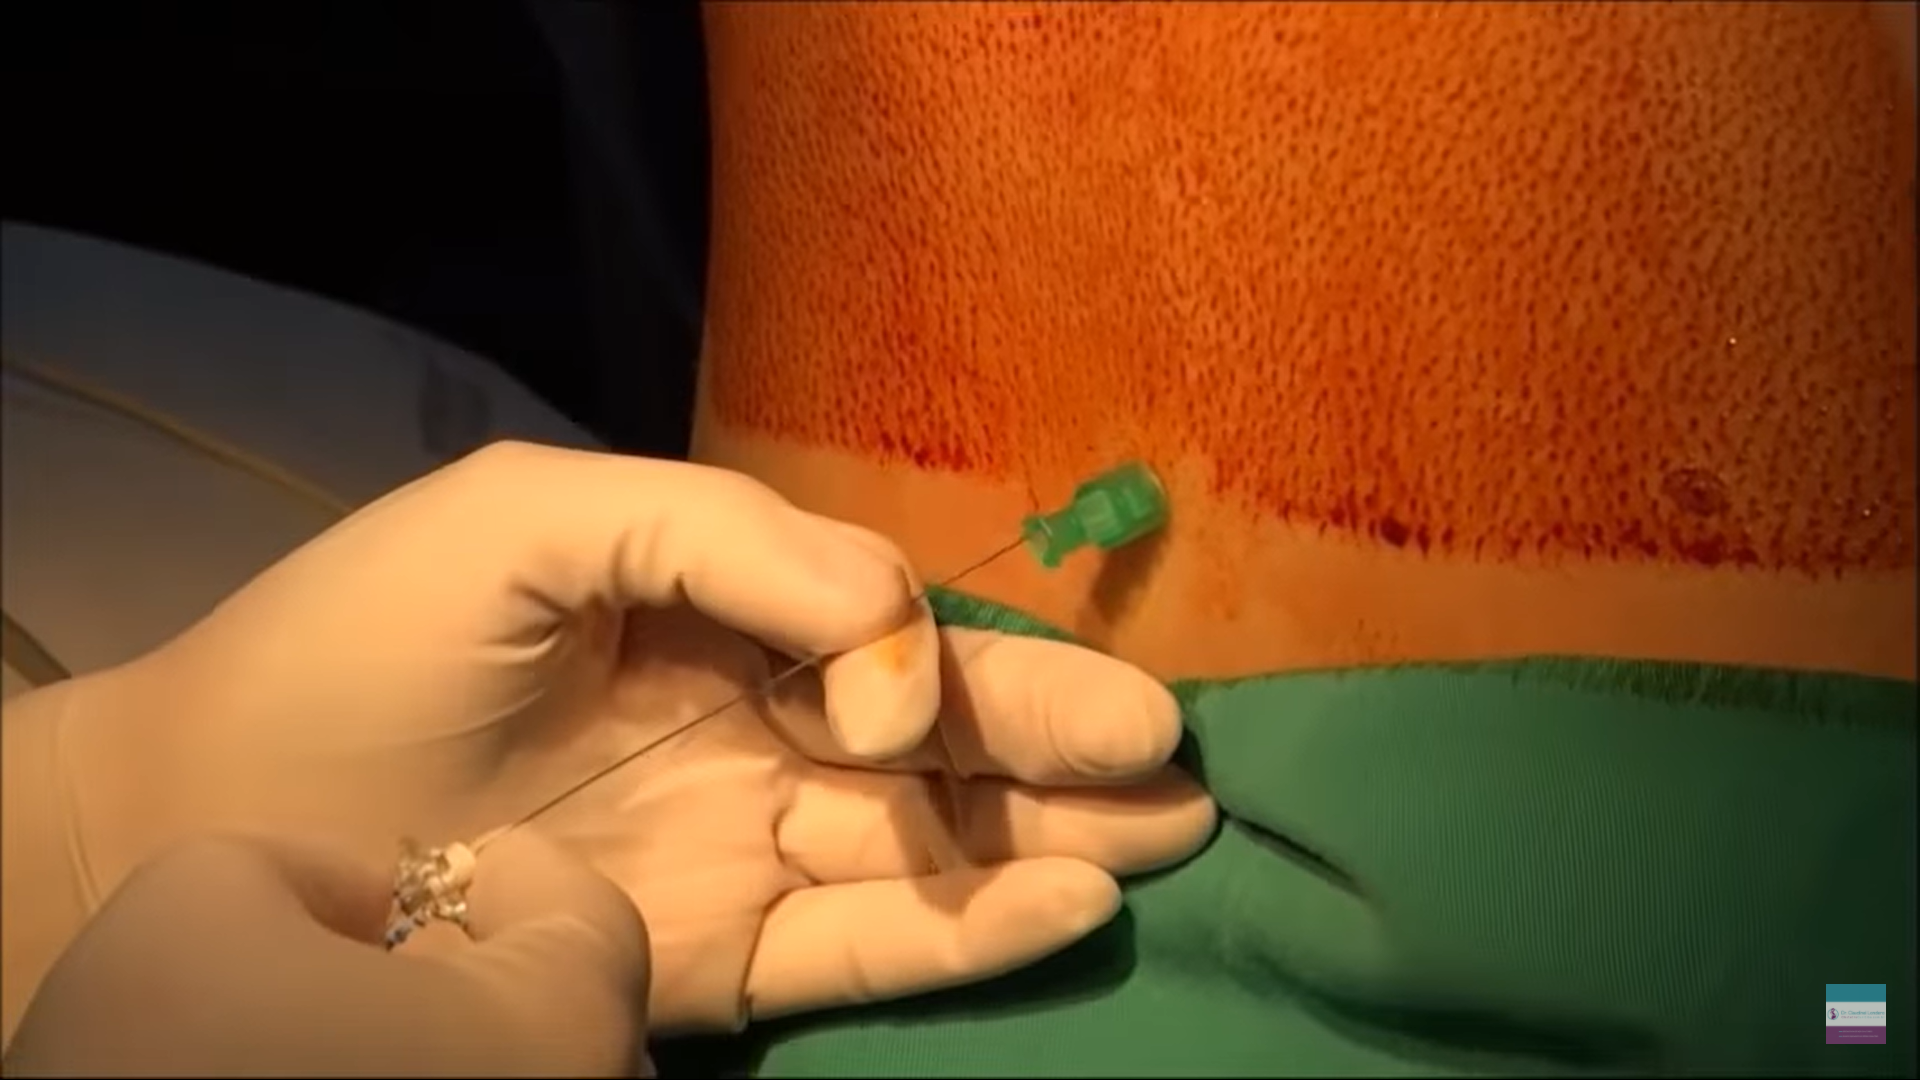
\includegraphics[scale=0.35,keepaspectratio=true]{figuras/2.PuncaoLombar.png} 
    \caption{Punção lombar com agulha de raquianestesia  \cite{Londero2018}.}
    \label{fig:puncaoLombar}
\end{figure}

\begin{figure}[h!]
    \centering
    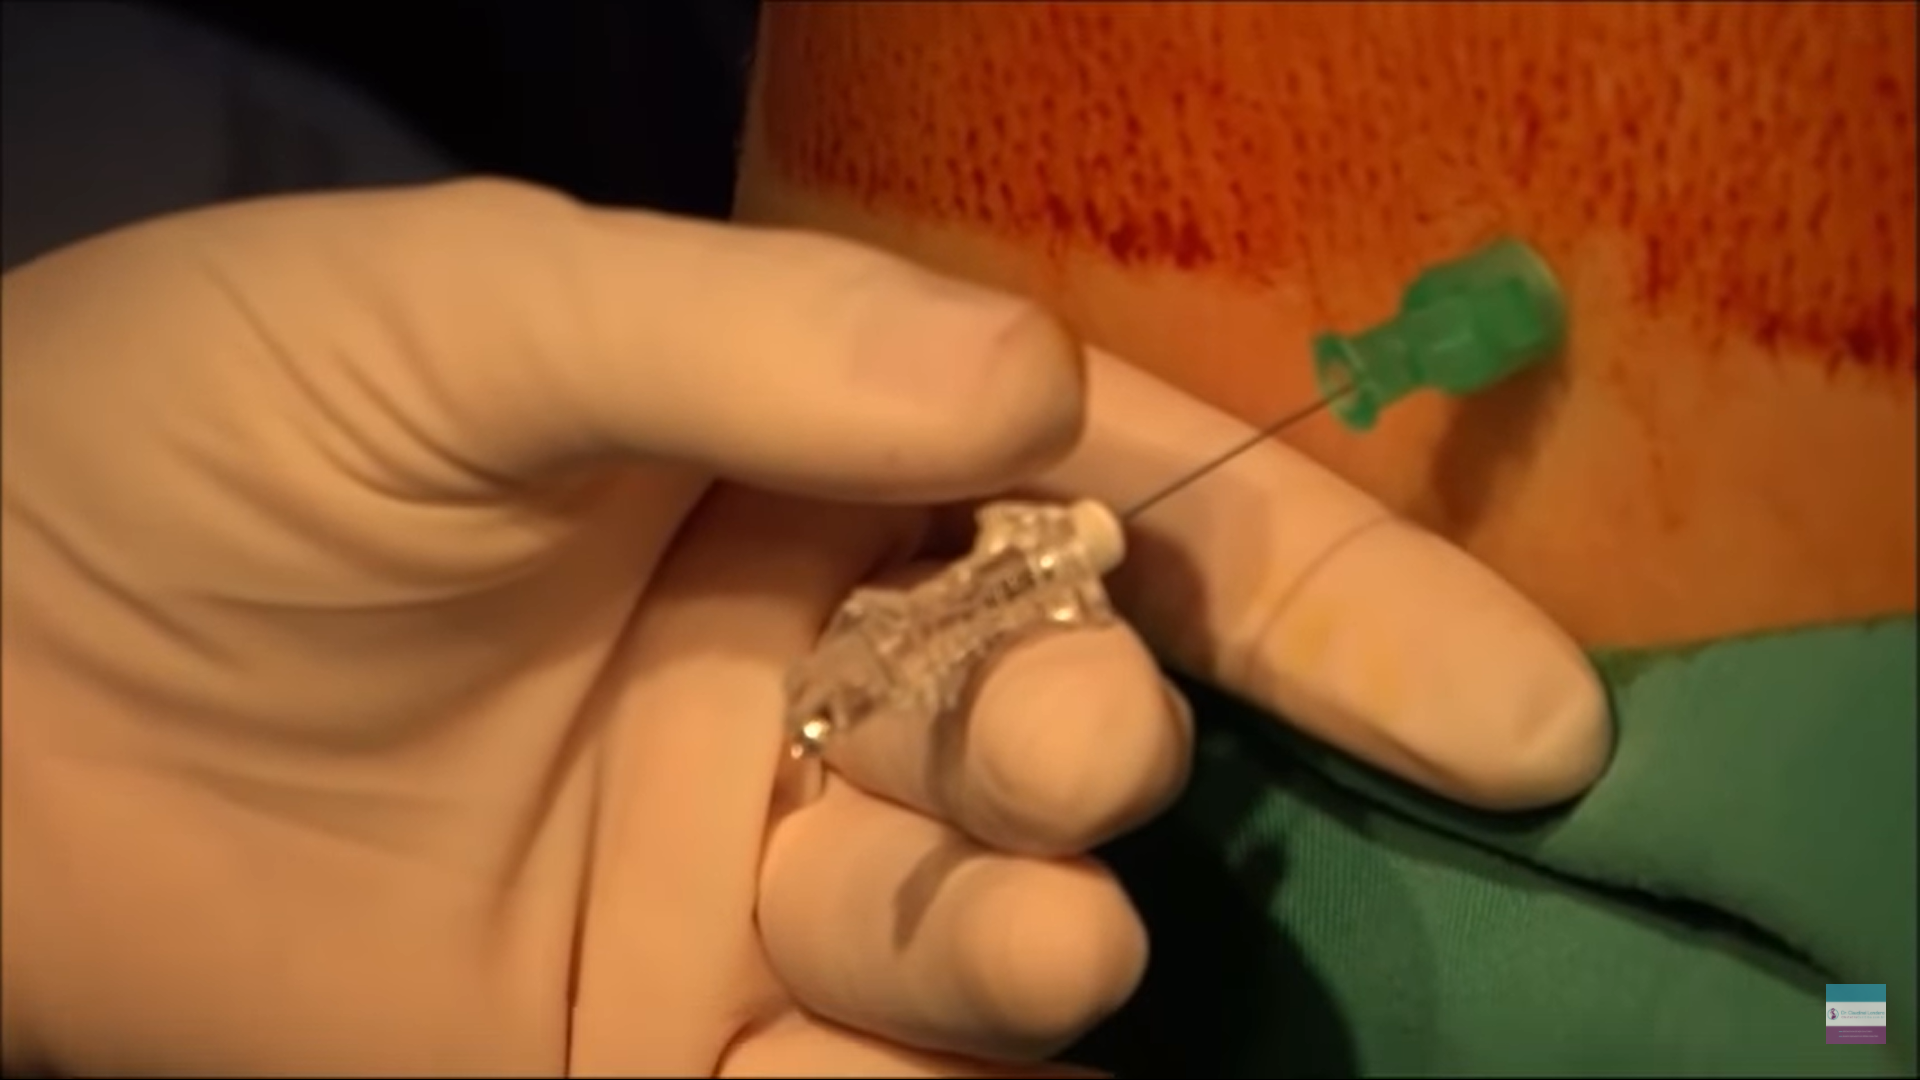
\includegraphics[scale=0.35,keepaspectratio=true]{figuras/3.GotejamentoLiquor.png}
    \caption{Gotejamento do \textit{líquor}, indicação do local correto para a raquianestesia \cite{Londero2018}.}
    \label{fig:gotejamentoLiquor}
\end{figure}

A principal abordagem de treinamento para técnicas de anestesia envolve a observação da aplicação das técnicas por anestesistas experientes. Estes orientam verbalmente os aprendizes conforme cada um dos passos é executado. Adicionalmente a isto são usados: desenhos 2D, cadáveres para demonstração do procedimento, apresentação de vídeos de procedimentos, visualização 3D e técnicas de simulação. No que diz respeito ao treinamento das sensações táteis além do treinamento em cadáveres alguns simuladores fazem uso de bonecos com tecidos artificiais \textit{phantoms} que simulam pacientes \cite{Dreifaldt2006}. Um ponto negativo importante no uso de \textit{phantoms} e de cadáveres, talvez o principal, é a baixa representatividade no que diz respeito a reprodução da situação real, pois estes oferecem uma baixa variabilidade de cenários (pacientes) para treinamento.  Outro aspecto relevante no uso de \textit{phantoms} é a necessidade de reposição de peças que se desgastam com o uso e podem ter custos altos. Estes são alguns dos motivos para que em diversos hospitais a primeira experiência do anestesista em treinamento seja efetuada diretamente em um paciente \cite{Aggarwal2009, Grantcharov2008, Smith2005, Watterson2007}. Esta prática, apesar de ser efetuada sob supervisão direta, traz riscos para estes pacientes e possíveis inseguranças aos aprendizes. 

O uso de simuladores para adquirir certo grau de habilidade antes de iniciar o procedimento em pacientes minimiza os riscos tanto para o aprendiz quanto para o paciente. O uso de simuladores com diversos cenários padroniza o ensino e possibilita ao aprendiz ter experiência com situações mais variadas.  Esta variabilidade de cenários dificilmente aconteceria na vida real em centros onde o ensino é feito diretamente em pacientes \cite{Udani2015}. Diversos simuladores utilizam dispositivos de força háptica (\textit{force feedback}) para auxiliar o aprendiz a experimentar fisicamente as sensações de resistência modeladas para os tecidos ao praticar procedimentos médicos. Este tipo de abordagem é usada em procedimentos médicos de um modo geral \cite{Escobar-Castillejos2016} assim como no caso mais específico dos procedimentos de anestesia \cite{Vaughan2013}. Existem inúmeras outras formas de como o uso de ferramentas computacionais podem auxiliar no campo da anestesia. Um exemplo é no controle automatizado de quanto anestésico aplicar a partir de respostas de medições dos níveis de consciência do paciente \cite{Mendez2009}.

\section{Ideia Central}


\section{Objetivos}
\label{sec:objetivos}



\section{Contribuições da Tese}
\label{sec:contribuicoes}



\section{Estrutura da Tese}
\label{sec:estrutura}

O restante do texto está estruturado da seguinte forma. O Capítulo~\ref{cap:cap2} comenta os principais conceitos e tecnologias envolvidas no desenvolvimento do ambiente de treinamento proposto.

O Capítulo~\ref{cap:cap3} contém os trabalhos relacionados a esta tese assim como o posicionamento deste trabalho frente aos demais.

No Capítulo~\ref{cap:cap4} é apresentada a proposta de desenvolvimento que foi desenvolvida durantes este trabalho. 

O Capítulo~\ref{cap:cap5} apresenta os experimentos que foram feitos. 

O Capítulo~\ref{cap:cap6} apresenta uma avaliação dos experimentos em relação aos seus resultados.

Por fim, o Capítulo~\ref{cap:cap7} conclui o trabalho, apresentando as conclusões, realçando as contribuições desta tese e apontando os  trabalhos futuros.
\chapter{Fundamentação Teórica} \label{cap:cap2}

Este Capítulo relaciona os conceitos e as tecnologias envolvidas no desenvolvimento do ambiente de treinamento proposto. 

\section{Anestesias Regionais}

Anestesias são atualmente usadas em diversos procedimentos cirúrgicos na medicina tradicional com o intuito de bloquear temporariamente a capacidade do cérebro de reconhecer um estímulo doloroso. Esta prática visa permitir a execução de procedimentos invasivos por parte do médico enquanto mantém o conforto e a tranquilidade do paciente. A anestesia regional é um procedimento usado em cirurgias onde o paciente pode permanecer acordado. Este tipo de anestesia bloqueia a dor em apenas uma determinada região do corpo, como um braço, uma perna ou toda região inferior do corpo, abaixo do abdômen \cite{Pinheiro2018}.

Os dois tipos de anestesias regionais mais usados são: anestesia raquidiana (ou raquianestesia, raqui), e anestesia peridural ou epidural. Estes dois tipos de anestesias também são conhecidas como anestesias de neuroeixo ou ainda bloqueio de neuroeixo \cite{Pinheiro2018}. Ambas podem ser aplicadas com pacientes sentados e inclinados para frente ou deitados de lado \cite{Anesclin2019}. 

\begin{figure}[h!]
    \centering
    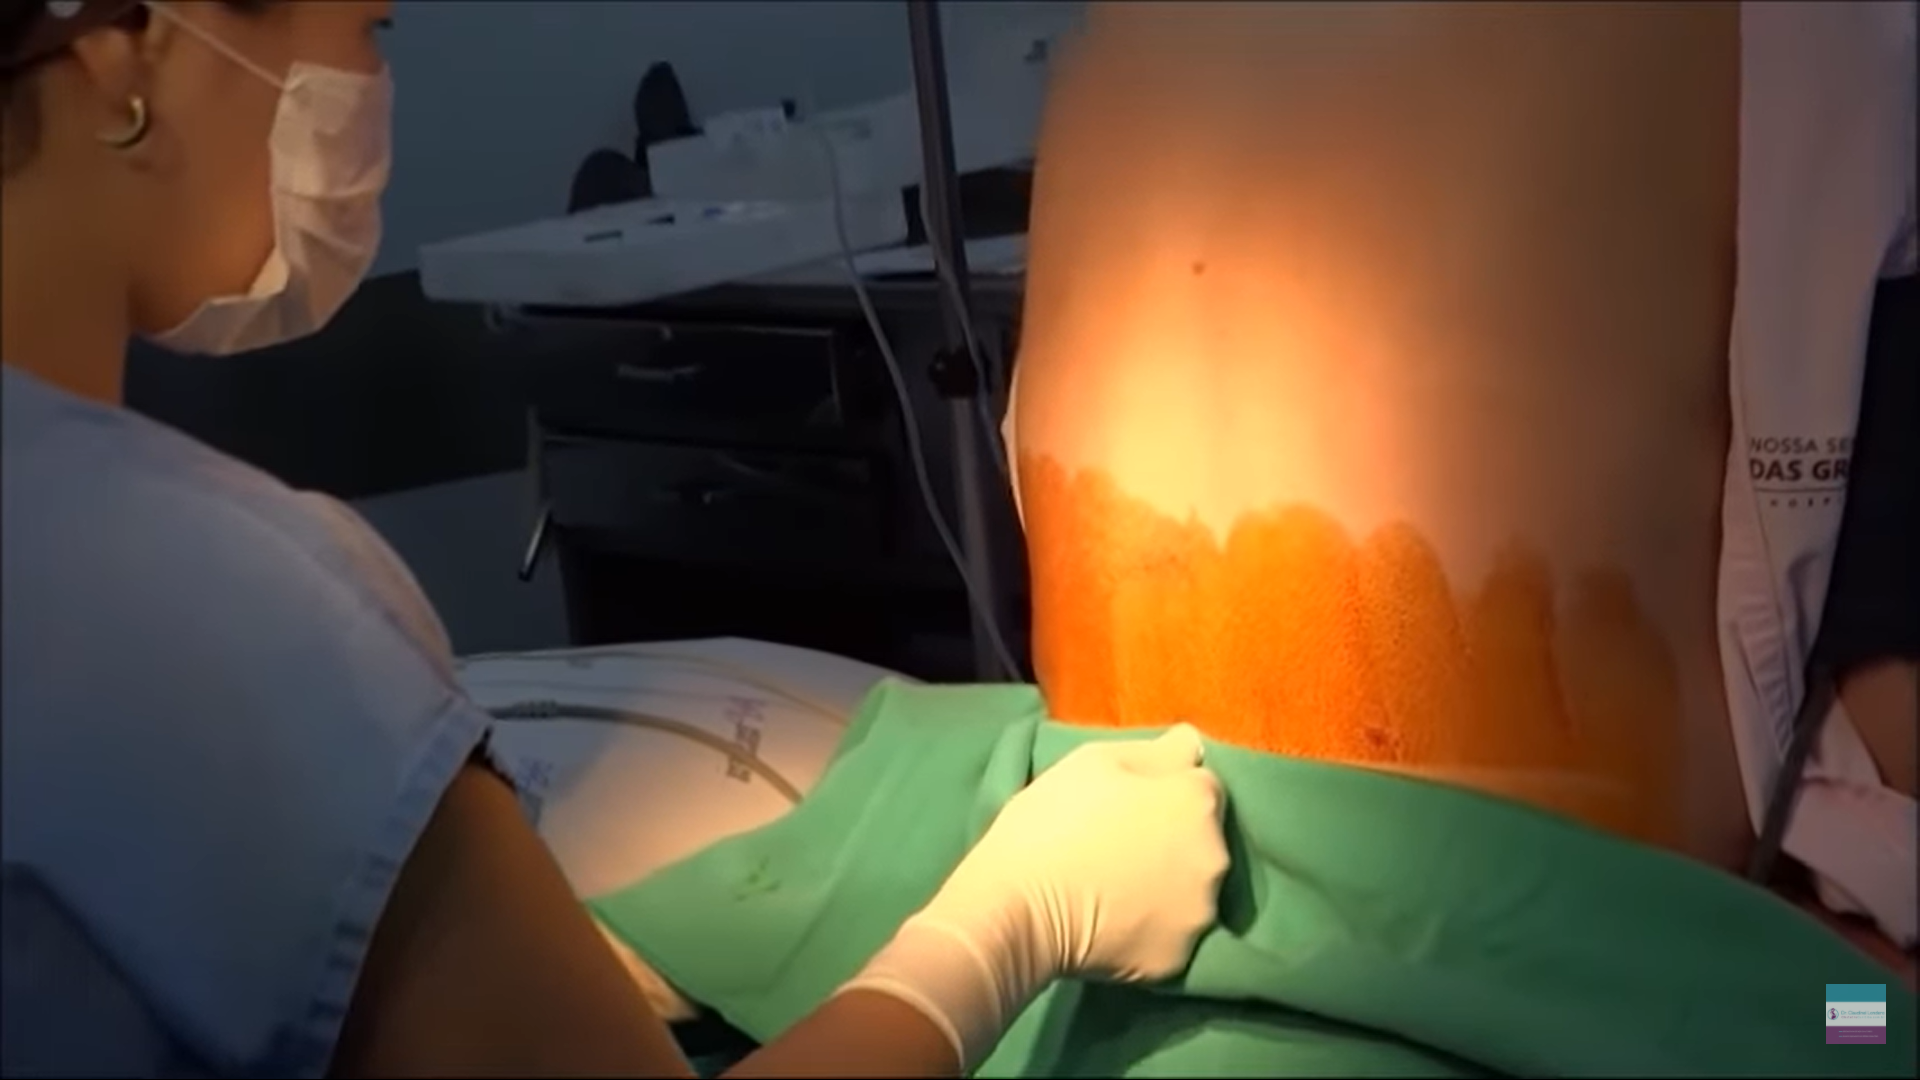
\includegraphics[scale=0.35,keepaspectratio=true]{figuras/0.marcacaoPonto.png}
    \caption{Palpação para determinação do ponto de inserção da agulha \cite{Londero2018}.}
    \label{fig:marcacaoPonto}
\end{figure}

\begin{figure}[h!]
    \centering
    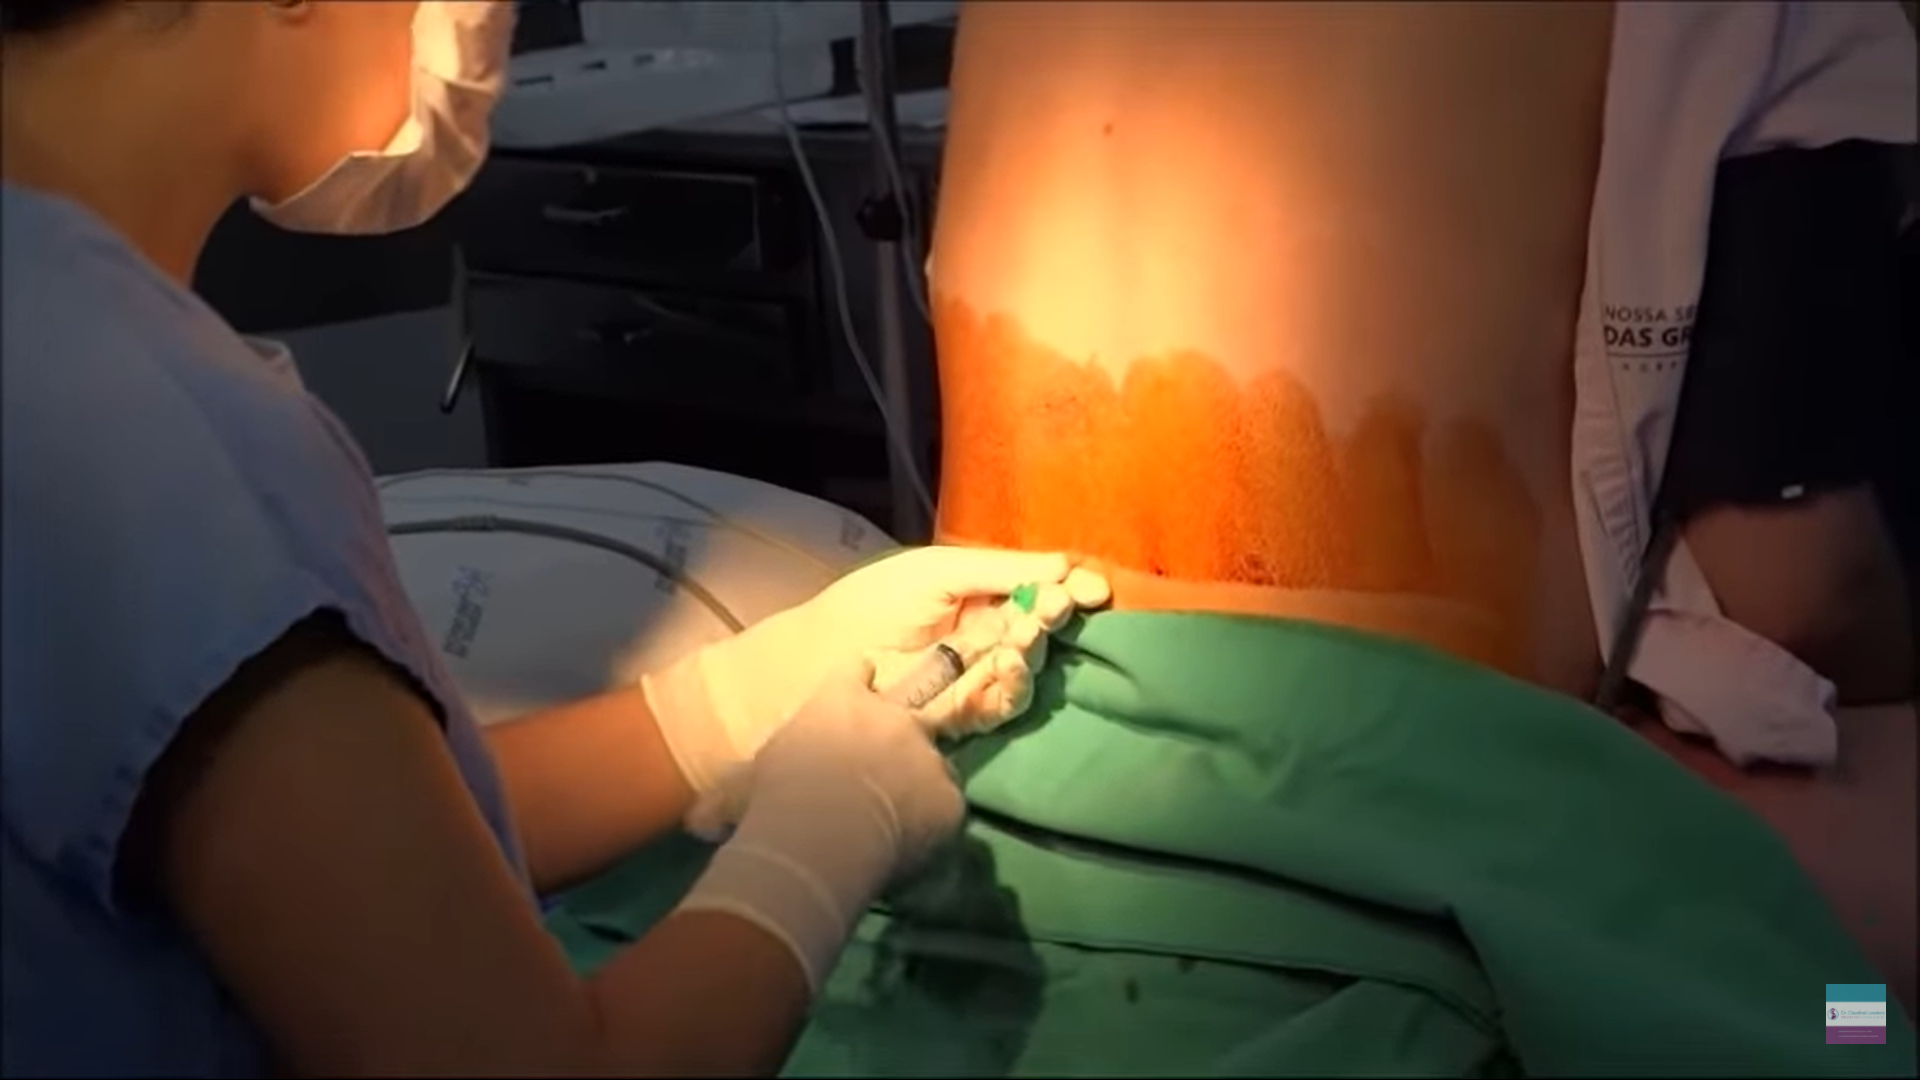
\includegraphics[scale=0.35,keepaspectratio=true]{figuras/1.AnestesiaLocal.png}
    \caption{Aplicação da anestesia local \cite{Londero2018}.}
    \label{fig:anestesiaLocal}
\end{figure}

\begin{figure}[h!]
    \centering
    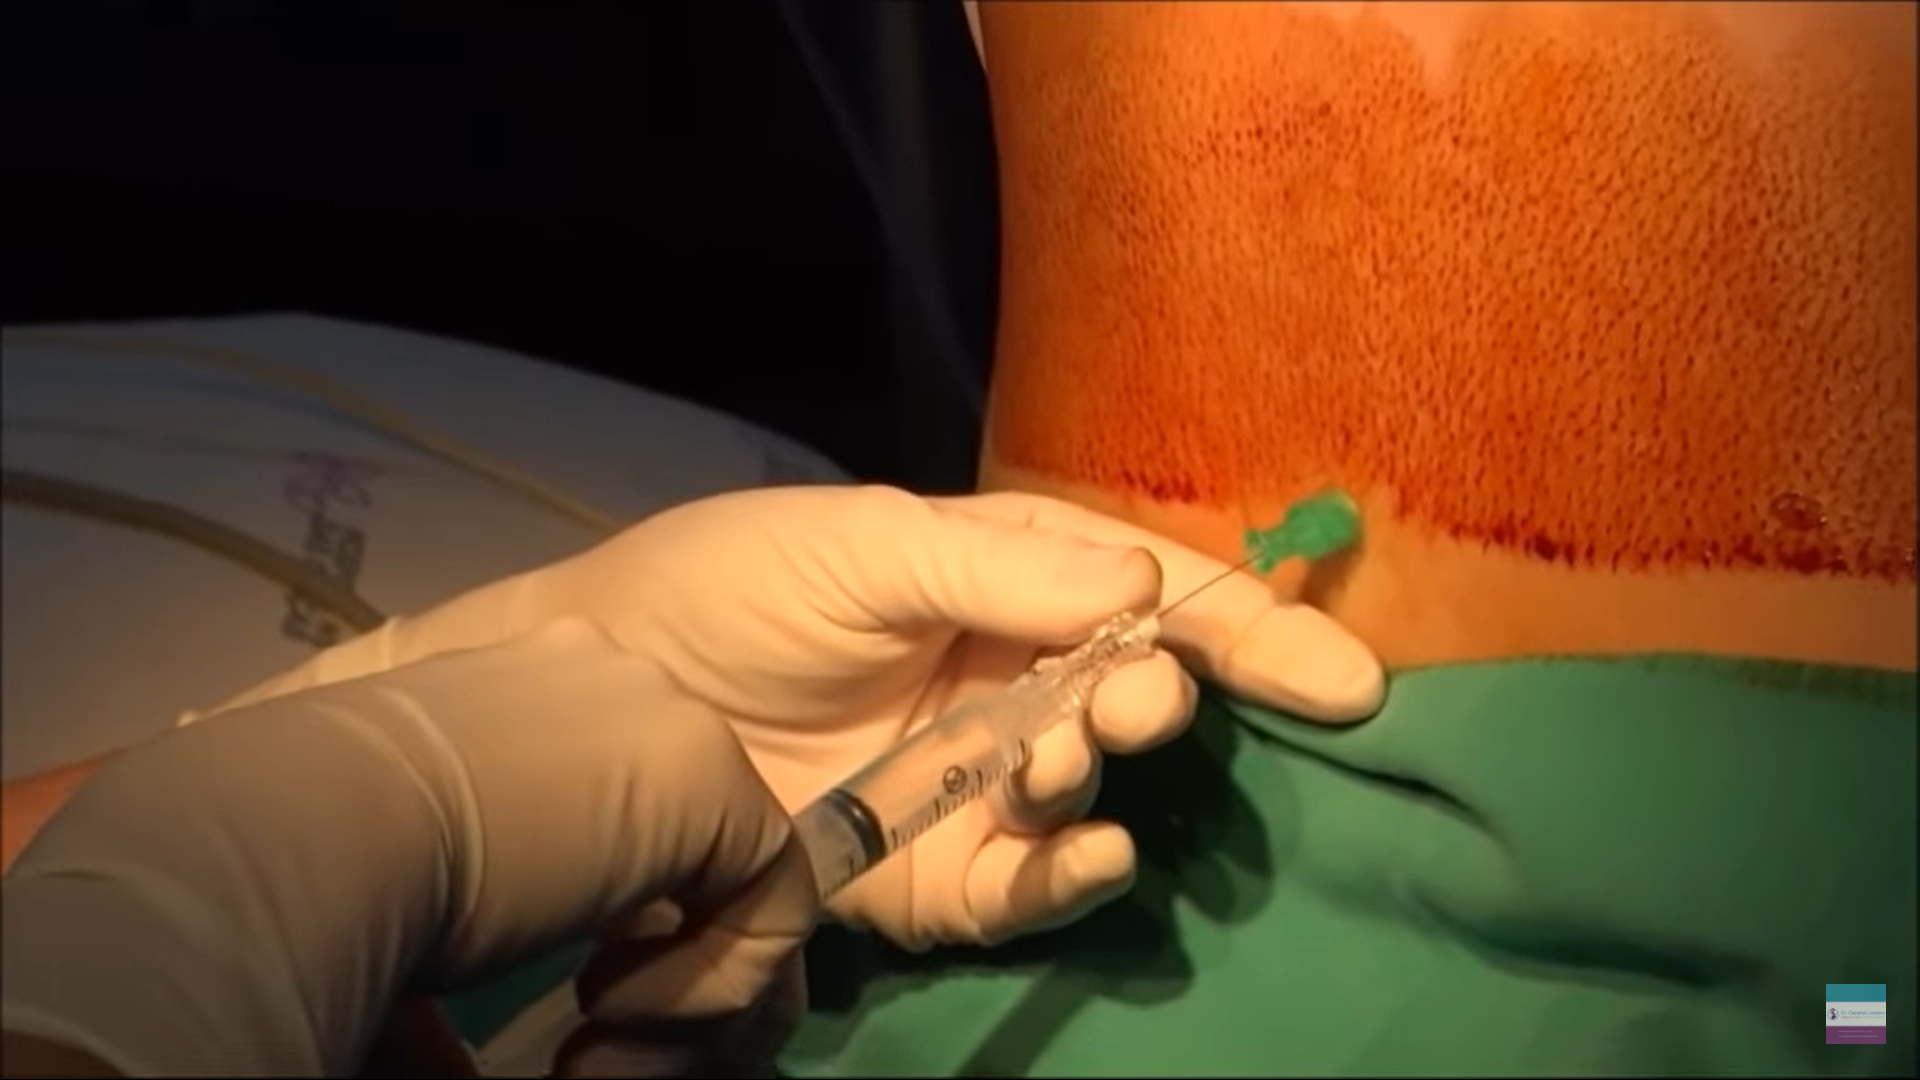
\includegraphics[scale=0.35,keepaspectratio=true]{figuras/4.InjecaoAnestesico.png}
    \caption{Injeção do liquido anestésico no espaço subaracnóideo  \cite{Londero2018}.}
    \label{fig:injecaoAnestesico}
\end{figure}

Após a finalização dos procedimentos de preparação é escolhida a área onde será feita a punção através do toque da mão do médico (exemplo retirado de video na Figura~\ref{fig:marcacaoPonto}) na crista ilíaca do paciente \cite{Helayel2010,Isaacs2015}. Uma vez escolhido este ponto é feita a injeção de anestésico local (Figura~\ref{fig:anestesiaLocal}) para reduzir o desconforto na área próxima à punção \cite{Sedicias2018} Após a anestesia local é feita a inserção da agulha de punção tanto no caso da peridural como na raqui.

Existem duas principais abordagens de inserção da agulha para efetuação das anestesias regionais. Estão são denominadas mediana (do inglês \textit{midline}) e paramediana (do inglês \textit{paramedian}). A abordagem mediana é utilizada com mais frequência (96\%) \cite{Wantman2006}. Um dos motivos para o maior uso da abordagem mediana é a ausência de vasos sanguíneos no caminho da agulha nesta abordagem \cite{Bapat2015}. A abordagem paramediana é mais recomendada para pacientes idosos \cite{Ahsan-ul-Haq2005} por motivos de modificação degenerativa da coluna vertebral \cite{Boon2003} e calcificação dos ligamentos interespinhoso e supraespinhoso \cite{Wantman2006}. A abordagem paramediana também pode ser mais viável que a mediana em pacientes obesos pela dificuldade na identificação da crista ilíaca nestes pacientes. Isto por que a camada de gordura faz com que a linha média seja mais difícil de localizar através do toque do médico \cite{N.2013}. Na abordagem mediana a agulha é inserida na linha média da coluna vertebral. Na paramediana existe certa angulação entre a linha da coluna e a inserção da agulha. As duas abordagens podem ser observadas no corte transversal da coluna na Figura 2 \cite{MedBroadcast2018}. 

===== FIGURA ====

\subsection{Anestesia Raquidiana}

Neste tipo de anestesia, uma agulha de pequeno calibre é inserida nas costas do paciente até atingir o espaço subaracnóideo (localizado após a dura-máter), dentro da coluna espinhal. Em seguida, um anestésico é injetado dentro do líquido cérebro espinhal (líquor), produzindo dormência temporária e relaxamento muscular (Figura~\ref{fig:injecaoAnestesico}). Anestesias raquidianas são aplicadas de forma mais frequente em espaços intervertebrais abaixo da segunda vértebra lombar (L2) (WIKIPEDIA, 2019). A Figura 3 ilustra em um corte sagital da coluna as diferentes camadas que são cruzadas por uma agulha durante o procedimento de punção lombar até chegar ao espaço subaracnóideo. Considerando as duas abordagens de inserção da agulha (mediana e paramediana) as camadas onde a agulha pode passar desde a pele até o espaço subaracnóideo são: gordura subcutânea, músculo, ligamento supraespinhoso, ligamento interespinhoso, ligamento amarelo (\textit{flavum}), espaço epidural e dura-máter. O processo espinhoso que também aparece entre a pele e o espaço subaracnóideo na Figura 3 não foi listado, pois, por ser uma camada de osso, ela não é perfurada pela agulha e sim uma camada intransponível em relação ao processo de punção.

A ação do anestésico dentro da coluna espinhal é a de bloquear os nervos que passam pela coluna lombar, fazendo com que os estímulos dolorosos vindos de membros inferiores e do abdômen não cheguem ao cérebro. A raquianestesia é muito usada para procedimentos ortopédicos de membros inferiores assim como na região abdominal e cirurgias obstétricas de parto normal e cesarianas \cite{Pinheiro2018}.

A grande vantagem da anestesia raquidiana em relação a peridural é que nesta é necessário o uso de uma pequena quantidade de anestésico local. Esta característica reduz consideravelmente o risco de intoxicação por meio do elemento anestésico. Por outro lado a maior desvantagem no uso deste tipo de anestesia está na dor de cabeça que os pacientes sentem após a perfuração da dura-máter. Este sintoma é causado pela lesão na dura-máter que pode permanecer aberta por alguns dias após o procedimento, provocando perda do líquor do espaço subaracnóideo. Com o uso de agulhas de menor diâmetro a incidência desta dor de cabeça foi consideravelmente reduzida \cite{INFOESCOLA2018}. 

===== FIGURA ====

\section{Realidade Virtual}

A realidade virtual está presente quando se usa a tecnologia para criar a ilusão de que se está em um ambiente que não está lá ou não existe. Ela é uma aproximação da realidade experimentada por nós através dos nossos sentidos e sistemas de percepção. A nossa percepção da realidade vem através dos nossos sentidos. Portanto, uma vez apresentando aos sentidos às informações esperadas, sendo estas reais ou não, a nossa percepção da realidade irá se guiar por estes estímulos. Os sentidos mais comuns são visão, olfato, paladar, audição e tato. Porém também possuímos outros sentidos que afetam as nossas percepções do mundo, como por exemplo: o senso de equilíbrio, o sentimento de forças, pesos e deslocamentos sentidos por nossos membros \cite{VRS2018}.

Atualmente, a chamada realidade virtual (RV) utiliza um computador para criar um ambiente virtual tridimensional. A intenção é a de simular uma realidade apresentando os elementos desejáveis para os sentidos do usuário, visando cumprir um objetivo através da interação de um ou mais usuários com este ambiente. Estes usuários se tornam parte deste ambiente virtual, total ou parcialmente, podendo manipular objetos ou executar um conjunto de ações \cite{VRS2018}.

A RV possui uma série de usos sociais como, por exemplo, o tratamento de fobias. Há trabalhos para aracnofobia \cite{Carlin1997}, para aicmofobia ou medo de agulhas \cite{Galoustian2018}, para aerofobia ou medo de voar \cite{Rothbaum2006}, para acrofobia ou medo de altura \cite{Edwards2018} ou de forma mais geral para o medo e a ansiedade \cite{Goldman2017}. A Figura 5 ilustra a aplicação para tratamento da acrofobia. Em primeiro plano a usuária com os óculos de realidade virtual e no segundo plano o ambiente virtual simulando ambientes de escadas e plataformas com fundo transparente.

===== FIGURA ====

A indústria do entretenimento através de filmes e jogos provocou uma grande evolução de técnicas de RV que posteriormente foram aplicadas em áreas mais “sérias” como o desenvolvimento pessoal/treinamento \cite{Ma2011, Prensky2001, Smith2011}. Na prática a RV deve ser considerada como uma possibilidade sempre que o que se deseja fazer é muito perigoso, caro ou impraticável de ser realizado concretamente. Por conta destas características ela é muito usada nas áreas da educação, da saúde e militar \cite{VRS2018}. Conforme a tecnologia que permite a criação e simulação de ambientes virtuais se torna mais barata, mais aplicações são criadas com o uso destas ferramentas.

\section{Dispositivos Hápticos}

O termo \textit{haptics} é usado para descrever a ciência que estuda e simula a pressão, textura, vibração e outras sensações biológicas relacionadas ao toque. A sensação do toque se origina em estímulos mecânicos, elétricos, térmicos ou químicos na pele \cite{Burdea1996}. O tato não está localizado numa região específica do corpo como os demais sentidos. Ele está distribuído por todo o corpo através do órgão sensorial do toque, nossa pele, articulações, músculos e tendões. O senso do toque se divide em duas sensações: cinética e tátil. Forças e torques são sensações cinéticas que sentimos nos músculos, tendões e articulações. Já as sensações táteis como pressão, deformação e vibração são sentidas por mecano receptores que possuímos na nossa pele \cite{Culbertson2018}. 

Os primeiros dispositivos hápticos foram originados dos braços robóticos usados para o controle remoto de robôs \cite{Zurawski2005} As aplicações de tecnologias hápticas são muito variadas envolvendo, por exemplo, projetos de engenharia e aplicações de manufatura \cite{Sharma2001}, entretenimento (videogames e filmes), celulares, relógios inteligentes e até mesmo a indústria automobilística \cite{Smith2019}. Estes dispositivos possuem elementos mecânicos de entrada e saída para interação com o usuário. Uma ou mais partes do dispositivo em contato com o usuário são monitorados no espaço físico e o dispositivo oferece como retorno força e torque. Desta forma um canal bidirecional de interação entre o ambiente virtual e o usuário é criado \cite{Coles2011}. Estes dispositivos estão sendo cada vez mais utilizados hoje em dia tanto pela evolução da sua tecnologia como pela diminuição dos preços. Com o avanço da tecnologia estes dispositivos estão se tornando cada vez mais flexíveis representando mais fielmente os movimentos. Isto ocorre  através do uso de conceitos de restrição parcial a movimentos, deslocamentos e da inclusão de mais graus de liberdade (\textit{degrees of freedom - DoF}). 

O número de graus de liberdade de um dispositivo háptico se refere ao número de maneiras diferentes em que este pode se mover ou criar forças. Como exemplo, dispositivos com 3 graus de liberdade podem rastrear posições e criar forças ao serem movidos nas direções: direita-esquerda, frente-trás e cima-baixo \cite{HAPTICSHOUSE2019}. O principal objetivo no uso destes dispositivos é o aumento da sensação de imersão em um ambiente de realidade virtual. 

Em relação à área médica, os dispositivos hápticos vem sendo utilizados na maioria dos trabalhos de simulação de procedimentos médicos \cite{Coles2011,Escobar-Castillejos2016}. Eles são usados para simular o uso de ferramentas em cirurgias e ajudaram a impulsionar o sucesso das práticas em simuladores virtuais. Isto aconteceu ao proporcionar o controle dos graus de liberdade de deslocamentos, a restrição aos movimentos e as respostas às atitudes do usuário como forças de reação ou feedback \cite{Gerovich2004}. Estes dispositivos eletromecânicos existem nas mais diversas formas e são adaptados para uma grande variedade de procedimentos médicos como, por exemplo, no treinamento de laparoscopia \cite{Srinivasan2004}, biopsia de próstata \cite{Sclaverano2009}, cirurgia de fígado \cite{Mastmeyer2016}, exames de mama \cite{Brazil2017,Jeon2010,Ribeiro2014,Solanki2010}, simulação de apalpação \cite{Ribeiro2016} e punções epidurais \cite{N.2013, Brazil2018}. Alguns sistemas usam mais de um háptico como em punções de agulha guiadas por ultrassom que usam um equipamento para simular a agulha e outro para o ultrassom \cite{Ni2011,Vidal2008}. Outros chegam a fazer o uso de três dispositivos como o PalpSim de forma a simular o toque das mãos do usuário num paciente virtual \cite{Coles2011b}. 

Culbertson et al. identificaram como 3 as principais categorias de sistemas hápticos: compreensíveis, vestíveis e palpáveis. Um exemplo visual destes tipos pode ser visto na Figura 6. Os sistemas compreensíveis são dispositivos tipicamente cinéticos (\textit{feedback} de força) que normalmente possuem uma base fixa e permitem ao usuário empurrar e ser empurrado de volta. Sistemas vestíveis são tipicamente táteis montados nas mãos ou em outras partes do corpo e provocam sensações diretamente na pele. Os sistemas palpáveis são dispositivos de encontro que permitem ao usuário explorar toda a superfície \cite{Culbertson2018}. Os dispositivos a serem explorados aqui são os de sistemas compreensíveis. Estes foram os tipos de hápticos utilizados nos simuladores computacionais relacionados ao tema desta tese (seção 0) assim com nos diversos outros simuladores médicos estudados e citados nesta seção. Ribeiro et al. fizeram uma revisão sobre dispositivos usados na simulação de procedimentos que envolvem o toque da mão do médico para identificação de características e anormalidades sob a pele \cite{Ribeiro2016}. Os autores analisaram 57 trabalhos e mais da metade fez uso dos dispositivos da família \textit{Phantom}. Os dispositivos desta família serão listados na seção ===== 3 ======.

===== FIGURA ====

Nas figuras Figura 7, Figura 8, Figura 9 e Figura 10 os dispositivos aparecem representados ordenados pelas suas complexidades i.e. dos mais simples (mais antigos e com menos recursos) aos mais avançados (mais novos). Todos estes dispositivos são exemplos de sistemas tipicamente cinéticos. Os mais novos possibilitam maior número de graus de liberdade para os movimentos assim como possibilitam mais forças e momentos de reação. O Novint Falcon ® (Figura 7), lançado em 2007, tem como interface com o usuário uma esfera onde o usuário deve colocar os dedos da mão para fazer os movimentos no caso do seu uso mais comum. No que diz respeito à liberdade de movimento este mecanismo proporciona uma interação 3D com o computador no lugar da interação 2D proporcionada pelo mouse. Ele possui 3 graus de liberdade de movimento e de forças. Nesta esfera existem quatro botões para interação e existem sensores para determinar a posição do cursor e motores para controlar as forças a serem transmitidas para o usuário. Existem versões onde a esfera é substituída, por exemplo, por um dispositivo semelhante a uma pistola para que o dispositivo seja usado em jogos de tiros de primeira pessoa \cite{VRS2017}. 

===== FIGURA ====

Os hápticos da família \textit{Phantom Geomagic Touch} ® (Figura 8) e \textit{Geomagic Touch} X ® (Figura 9) apresentam uma peça que simula uma caneta para manipulação do usuário da mesma forma que a esfera no dispositivo da Figura 7. Nas canetas também existem botões para interação e da mesma forma estas também são substituíveis por partes com formas mais adequadas ao procedimento que estas pretendem simular. O dispositivo \textit{Geomagic Touch} X ® possui a mesma liberdade de movimento do \textit{Geomagic Touch} ®, porém possibilita \textit{feedback} de reações maiores. Ambos apresentam 6 graus de liberdade de movimento e 3 graus de liberdade no retorno de forças. Estes dispositivos, portanto mapeiam a posição 3D e orientação, mas somente apresentam \textit{feedback} de forças direcionais \cite{Forsslund2013}.

===== FIGURA ====

===== FIGURA ====

O \textit{Phantom Premium} ® (Figura 10) está disponível nas versões \textit{Premium} 1.0, \textit{Premium 1.5} e 1.5/HF, e \textit{Premium} 3.0. Estas evoluem não só o \textit{feedback} de reações como também os graus de liberdade dos movimentos. Enquanto o \textit{Phantom Premium} 1.0 ® simula o movimento do giro do pulso na mão o \textit{Phantom Premium} 3.0 ® possibilita uma amplitude que simula os graus de liberdade de movimento de todo o braço humano desde o ombro \cite{3DSystems2018}. Este dispositivo possui 6 graus de liberdade tanto para movimento como retorno de forças o que o torna simétrico no número de sensores e motores (atuadores). São computadas forças e torques tanto da posição como da orientação deste dispositivo. Esta característica tem uma forte influencia no alto custo associado a este tipo de dispositivo \cite{Forsslund2013}.

===== FIGURA ====

=========

\section{Modelagem de tecidos}

Um dos passos necessários para construção de um ambiente virtual para treinamento de anestesia epidural e raquianestesia é a criação de pacientes virtuais. Um importante aspecto da modelagem destes pacientes é como eles aparecem na tela da aplicação. Outro aspecto importante na simulação é ter uma estimativa da espessura dos tecidos envolvidos nestes tipos de anestesia. Para isto é necessária à modelagem do tamanho de todas as camadas de tecido pelos quais as agulhas passam para execução destes procedimentos. Uma ilustração destes tecidos que vão desde a pele até a dura-máter pode ser vista na Figura 3. Nesta seção são descritos trabalhos relacionados com a modelagem da distância entre a pele e a dura-máter.

Na Tabela 2 são listadas as varáveis de entrada e saída dos métodos estudados nesta seção. Esta tabela exibe também as unidades destas variáveis que serão utilizadas em todo este trabalho.

===== TABELA ====

Muitos trabalhos buscam relacionar a distância que vai da superfície externa da pele até o espaço epidural (DEE) com as demais variáveis da Tabela 2. A grande maioria dos trabalhos indica uma forte relação da DEE com o IMC \cite{Adegboye2017, Galbraith2018}. Estes dois trabalhos não fazem separação dos grupos populacionais por idade, sexo ou etnia, e usaram populações respectivamente de n=120 e n=317 pessoas entre homens e mulheres.

Os trabalhos citados a seguir analisaram somente ou de forma separada grupos de mulheres grávidas. Como este é o foco deste trabalho só serão comentadas aqui as conclusões referentes a estes grupos. Todos os trabalhos a seguir encontraram influencia do IMC na determinação da DEE, mas além desta relação também foram encontradas outras combinações em cada trabalho. O grupo étnico/populacional do individuo foi observado em conjunto com o IMC em \cite{Sharma2011} estudo feito no Reino Unido. A idade foi observada em conjunto com o IMC num estudo em pacientes americanas em Michigan, EUA \cite{Clinkscales2007}. A altura, massa, idade e IMC foram observados como relevantes em um estudo em pacientes da Índia \cite{Hazarika2016}. Estes dois últimos trabalhos construíram equações de regressão linear para determinação da DEE para grupos de parturientes conforme pode ser visto na Tabela 3.

===== TABELA ====

Os autores em \cite{Sharma2011} no lugar das equações apresentaram como resultado uma tabela com cinco pontos de cada par IMC x DEE para cada grupo populacional analisado. Estes dados podem ser vistos na Tabela 4. A definição dos grupos populacionais no estudo do Reino Unido (RU) em \cite{Sharma2011} foi: Brancas (população do Reino Unido, da Irlanda e qualquer outro grupo com cor de pele branca); Asiáticas ou Britânicas Asiáticas (população da Índia, Paquistão, Bangladesh ou qualquer outro grupo Asiático); Negras ou Britânicas negras (população de Africanas, Caribenhas ou outros grupos com cor da pele negra); e Chinesas e outros grupos étnicos (população da China, Japão, Malásia, Filipinas etc.). No grupo de nome Chinesas, além dos dados de pessoas desta origem moradoras do Reino Unido, foram considerados dados de Chinesas (n=70) de um hospital de Singapura.

===== TABELA ====

Na Tabela 5 é apresentado o tamanho da população utilizada nestes estudos e as identificações da origem dos dados do estudo, isto é, os grupos populacionais analisados. 

===== TABELA ====

A listagem dos tecidos entre a pele e a DEE e a relação dessa distância com o aumento de peso é comentada em \cite{Palmer1983}. Os autores concluem que com o aumento do peso/massa (do paciente) o tecido que sofre a maior variação é a gordura subcutânea.

Na seção = ==== é proposto o uso de dados de trabalhos comentados aqui para modelagem de tecidos de pacientes grávidas.

=========

Este capítulo apresentou uma fundamentação teórica sobre ====. Iniciou apresentando ==========. Logo em seguida o capítulo apresenta ====== e suas principais entidades e que estão relacionadas com a proposta desta tese. O capitulo finaliza apresentando os conceitos que envolvem ==== e seus principais elementos. O próximo capítulo oferece uma visão das pesquisas relacionadas ao tema desta tese e compara-as com as proposições que foram colocadas ao longo deste trabalho. Essas pesquisas tratam e ========== assim como de ===========.
\chapter{Trabalhos Relacionados} \label{cap:cap3}

Os trabalhos apresentados neste capítulo vão desde abordagens para definição e classificação de multimodalidade  \cite{turunen2009multimodal}, propostas como \cite{guedes2016extending} de uma especificação de interação multimodal e multiusuário, apresentações de padrão como em \cite{Kim:2014aa} com o Padrão MPEG-V, implementações que provem integração de sistemas em \cite{pereira2017middleware} integrando o Ginga-NCL com M-HubM-Hub \cite{talavera2015mobile} até trabalho como \cite{mcgill2015review} que discute e importância e os desafios encontrados para implementação de um TV multi-usuários.  

\section {Multimodalidade}

Normalmente, os sistemas de televisão digital permitem o controle sobre o conteúdo transmitido por meio do Guia Eletrônico de Programação (EPG). O EPG consiste em uma grade, onde as colunas representam os canais de televisão, enquanto as linhas representam os intervalos de tempo. Nesse contexto, Turunen et al. \cite{turunen2009multimodal} descrevem como novas modalidades de interface de usuário podem ser usadas para fornecer vários métodos de entrada e saída para interação com o EPG. As modalidades de interação apresentadas em \cite{turunen2009multimodal} incluem gestos, entrada de fala e toque físico. A interface de gestos é usada junto com o teclado do telefone celular. Nesta modalidade de interação, diferentes orientações do celular mudam o funcionamento do teclado. Por exemplo, as teclas de seta vertical para baixo são usadas para mover a seleção no EPG e as teclas de seta horizontal executam funções de \textit{zoom}.

Em \cite{turunen2009multimodal}, a interação por voz inclui comandos para navegação no aplicativo (por exemplo, "Vá para o guia de programação") e para assistir à mídia ("Vá para o canal de notícias"). Os autores também fornecem uma interface de toque físico por meio de uma placa de controle semelhante a um controle remoto clássico, mas em vez de botões, ela possui etiquetas RFID atrás de ícones que se comunicam por meio de celular. Quando um usuário toca um desses objetos com um telefone celular, o comando é lido da tag e entregue ao sistema. De acordo com Turunen et al. \cite{turunen2009multimodal}, os ícones tornam o sistema mais fácil de usar do que um controle remoto clássico. Quando o usuário toca em qualquer ícone do controle, o comando associado é enviado ao EPG.

Na literatura, há diversas soluções propostas para trazer maior interatividade para o usuário, por meio do \textit{middleware} Ginga. Em especial pela adição de dispositivos que funcionem como uma segunda tela de interação com a TV \cite{nery2008desenvolvimento}. Dentre estas soluções, destaca-se a de Batista et al. \cite{batista2010estendendo}. Os autores propõem um módulo para o \textit{middleware} Ginga que possibilita aplicações NCL utilizarem recursos de outros dispositivos secundários para controlar a exibição de conteúdo, interação e captura de eventos. Além disso, a solução permite criar \textit{links} que são acionados de acordo com a identificação do dispositivo secundário. Um característica dessa solução é a utilização de uma API para gerenciamento e registro das classes de dispositivos que irão se comunicar com o dispositivo pai. Um caso de uso é a utilização de celulares para responder pesquisas, controlar a televisão e visualizar conteúdo em conjunto com a aplicação. É importante notar que nesse trabalho relacionado, não são sugeridas novas modalidades de interação, porém, foram lançadas as bases para o desenvolvimento de extensões ao Ginga.

O trabalho de Pedrosa et al. \cite{pedrosa2010componente} especifica e implementa um componente que  permite o recebimento de eventos multimodais por parte de aplicações em C++ residentes no Ginga. Na arquitetura proposta, módulos de comunicação devem enviar um documento XML contendo informações do evento, que por sua vez será traduzido por um \textit{parser} para um objeto, informando a um gerenciador de eventos para notificar as aplicações que manifestaram o interesse pelo evento. No trabalho de Pedrosa et al. \cite{pedrosa2010componente}, a principal contribuição foi utilizar o subsistema Ginga para dar apoio à notificação de eventos de multimodalidade para aplicações C++. Em contraste, no presente trabalho, é proposta uma arquitetura que permite que o tratador de eventos do Ginga reconheça também eventos provenientes de outras modalidade de interação. Com isso, possibilita que aplicações declarativas em NCL sejam construídas com multimodalidade. Além disso, este trabalho propõe a parametrização destes eventos de multimodalidade, de forma a permitir também a interação multimodal por múltiplos usuários.

O trabalho de Carvalho et al. \cite{carvalho2010estendendo} propõe uma arquitetura de software focada na interação entre o usuário e a televisão por meio de sua voz com comandos vocais simples, com o objetivo de substituir funções do controle remoto. Para permitir tais aplicações, os autores propõem diversos novos elementos na linguagem NCL, que são derivados da linguagem VoiceXML. A abordagem de extensão de NCL depende de modificações extensas no formatador da linguagem, porém, no trabalho não é especificado como o formatador deverá reagir. Além disso, não é especificado como o software de reconhecimento poderá ser acoplado ao Ginga-NCL.

Luque et al.\cite{luque2014integration} propõe a inserção de objetos 3D interativos na tela principal da televisão. Além disso, a proposta apresentada em \cite{luque2014integration} também permite a interação por meio de um dispositivo tátil portátil (ou seja, tela secundária). A segunda tela fornece informações adicionais, como estatísticas e visualizações adicionais apresentadas sob demanda. A proposta deles foi aplicada à TV interativa que é capaz de receber e reproduzir conteúdo proveniente de redes de difusão (como a televisão digital terrestre) e da Internet (ou seja, a rede de banda larga). É importante ressaltar que a interação multimodal proposta em \cite{luque2014integration} é caracterizada pela utilização de mais de um dispositivo de interação (joystick e tablet). Porém, em nossa proposta, a interação multimodal está relacionada ao uso de diferentes modos de interação, como voz, gesto ou reconhecimento do olhar.



Guedes et al. \cite{guedes2016extending} propõem uma estrutura de programação de alto nível para apoiar interfaces de usuário multimodais em aplicações multimídia interativas. O framework integra diferentes tipos de modalidades de entrada e saída. Ou seja, suporta modalidades de entrada geradas pelo usuário, como gestos e reconhecedores de voz, e modalidades de saída, como conteúdo audiovisual tradicional, sintetizadores de fala e atuadores. O trabalho modela tipos de entrada multimodais que suportam novas modalidades de entrada, tais como gestos e reconhecimento de voz, e diferentes modalidades de saída, como os conteúdos audiovisuais tradicionais, sintetizadores de voz e atuadores. Para o reconhecimento de voz, os trechos a serem reconhecidos são definidos por meio de arquivos SRGS (\emph{Speech Recognition Grammar Specification}) \cite{srgs}. O \textit{framework} proposto não foi implementado no Ginga-NCL. Essa proposta é bastante diferente da proposta desta tese, onde representam-se diferentes tipos de interação (voz, gesto, etc) através de  diferentes tipos de eventos NCM. Sendo assim, não é necessário criar novos tipos de nós e âncoras NCM para reconhecer a ocorrência desses eventos, como \textit{RecognitionNode} e \textit{RecognitionAnchor} propostos em  \cite{guedes2016extending}. Além disso, fica transparente para o autor o domínio da gramática utilizada pelos reconhecedores.

Pereira et al. \cite{pereira2017middleware} propõem uma infraestrutura de software que tem por objetivo integrar o Ginga-NCL\cite{ABNT:2011aa} com o M-Hub\cite{talavera2015mobile}, um middleware voltado ao domínio da IoT que permite a descoberta dinâmica, estabelecimento de conexão, acesso e distribuição de dados de/para objetos inteligentes. Uma limitação do trabalho é imposta pela limitação das informações que podem ser trocadas via script Lua pois é a única forma de capturar informações publicadas no \textit{broker}. O trabalho não propõe extensões na linguagem NCL de forma que o autor da aplicação possa tratar interações vidas dos dispositivos inteligentes.

Na proposta de Farias et al. \cite{de2020extensions}, o Ginga foi estendido com suporte ao MQTT, para prover integração entre IoT (\textit{Internet of Things}) \cite{gubbi2013internet} e TV digital (TVD). O trabalho desenvolveu aplicativos para validar a estrutura proposta utilizando comunicação MQTT em uma rede doméstica. Informações coletadas da rede doméstica por sensores puderam ser apresentadas na TV. Assim, o trabalho adiciona novos recursos ao \textit{middleware} Ginga, que permitiu a integração de receptores de TVD em aplicativos de IoT, por uma API desenvolvida em NCLua \cite{sant2008nclua}. Porém esta abordagem mantém uma dependência com scripts NCLua onde há uma limitação na troca de informações com as aplicações NCL.

\begin{comment}

\begin{table}[h]
\centering
{
  % distancia entre a linha e o texto
  \renewcommand\arraystretch{1.25}
  \begin{tabular}{|p{1,5cm}|p{6cm}|p{1,5cm}|p{2cm}|} \hline
   \multicolumn{1}{|c|}{Trabalho} & \multicolumn{1}{|c|}{Descrição} & \multicolumn{1}{c|}{Média (ms)} & \multicolumn{1}{c|}{Confiança} \\\hline
    1 & 1 usuário com 5 propriedades &  0  & 1,09E-09    \\\hline
    2 & 5 usuários com 5 propriedades &  1  & 2,04E-09   \\\hline
    3 & 10 usuários com 5 propriedades &  1  & 7,76E-10  \\\hline
    4 & 5 usuários com 10 propriedades &  1  & 1,06E-09  \\\hline
    5 & 10 usuários com 10 propriedades &  1  & 1,47E-09 \\\hline
   \end{tabular}
\caption{Tabela comparativa dos trabalhos relacionados a multimodalidade}
\label{tab:compMultimodalidade}
}
\end{table}
%
\end{comment}
\section {Multiusuário}

O trabalho de Guedes et al. apresentado em \cite{guedes2017extending} se concentra em questões de especificação de interações multiusuário. Mais precisamente, em como o autor define os requisitos de interação do usuário e usa informações de contexto. Não é abordado como o sistema de multimídia deve reunir a descrição do perfil dos usuários e a recuperação de suas variáveis de contexto de tempo de execução. Além disso, todas as características de todos os usuários são armazenadas em um único nó de propriedades do documento multimídia. Neste nó, é armazenado um vetor para cada propriedade que se deseja manter dos usuários. A proposta desta tese se aproxima da abordagem de \cite{guedes2017extending}, à medida que foi criado também uma entidade para representar a classe de usuários. Porém difere em alguns aspectos, pois foram criadas duas entidades para representar os usuários individualmente, uma para identificá-lo e outra para armazenar suas características, sendo representada por um nó de propriedades.



McGill et al. \cite{mcgill2015review} discutem o uso da TV e multitelas, os problemas que esse uso apresenta com relação ao papel da TV em contextos sociais compartilhados e o impacto potencial que novas tecnologias podem ter sobre como usamos e interagimos com a televisão. O uso compartilhado da TV é problemático, tanto do ponto de vista da interação quanto da incapacidade de usar a TV de forma independente, sem afetar o uso de terceiros. Atualmente, os usuários superam esses problemas por meio de várias telas, mas isso também é problemático do ponto de vista social, com potencial para aumento do isolamento digital e falta de compartilhamento com relação aos presentes. McGill et al. demonstram como esses problemas podem ser resolvidos com design de interação de TV, apresentando maneiras em que o uso multiusuário pode ser facilitado por meio de interfaces de uso compartilhado e multivisão, e examinando como a TV pode permitir maior compartilhamento e, portanto, consciência da atividade do dispositivo propondo dois tipos de interface. A interação mediada e a interação concorrente. Com isso, foi demonstrado que a TV é capaz de fazer substancialmente mais do que atualmente é solicitado; ao contrário do uso existente, pode ser de relevância crescente na era multiusuário e multitelas. Outra questão interessante discutida em \cite{mcgill2015review}, foi as possibilidades de que todos os usuários pudessem estar no controle da interação. Dentre elas: \textit{Subsets} onde diferentes membros do grupo tem o controle de diferentes funções exigindoa assim cooperação; \textit{Hierarchy} onde a interação de um mebro sobrepõe a do outro; \textit{plurality} a decisão da seleção são baseadas na maioria dos votos mas a navegabilidade é concorrente e finalmente \textit{Blocking} permite que membros possam bloquear temporariamente outro membro do cobtrole. Em todas as possiblidades  há necessidade a identificação do usuário e é neste ponto que o trabalho conversa com esta tese a medida que também há a identificação do "dono" da interação . Em \cite{mcgill2015review}, os autores não apresentam um arquitetura para prover interação multiusuário, mesmo porque o objetivo do artigo é mostrar como os comportamentos existentes para compartilhamento de uso podem ser reaproveitados e virtualizados.


\chapter{Proposta de Extensões ao Modelo NCM e à Linguagem NCL} \label{cap:cap4}

A Linguagem NCL \textit{Nested Context Language}) é baseada no modelo conceitual NCM (\textit{Nested Context Model}). Esta tese propõe extensões ao modelo NCM e à linguagem NCL para incluir as facilidades de interação multimodal e suporte multiusuário. As próximas seções detalham as extensões propostas.

\section{Extensões ao Modelo NCM}
\label{sec:NCMExt}

A extensão ao Modelo NCM (\textit{Nested Context Model}) proposta nesta tese se divide em duas partes. A primeira parte diz respeito a novas entidades NCM para suporte a múltiplos usuários, proposta que estende as ideias de \cite{guedes2016extending}, e também informações de contexto, considerando a abordagem apresentada em \cite{Josue:2018:MSE:3204949.3204967}. A segunda  parte diz respeito à criação de novos tipos de eventos no modelo NCM para dar suporte à interação multimodal, propondo uma abordagem diferente da proposta de \cite{guedes2016extending}. 

\subsection{Multiusuário}
\label{sec:MultUser}

Em relação à modelagem dos usuários que participam de uma experiência multimídia, diferente de \cite{guedes2016extending}, este trabalho representa um usuário individualmente com suas características específicas que poderiam, por exemplo, ser carregadas de um perfil especificado em uma arquivo XML no padrão MPEG-21 parte 22 \cite{ISO/IEC:2019aa}. As características podem conter desde preferências de tipos de mídia até limiares de percepções como volume de som, luminosidade, etc. 

Para representar os usuários individualmente de maneira especifica é proposta a entidade  \textit{userAgent}. Um \textit{userAgent} indica um único usuário e tem o atributo \textit{src}, que indica a especificação de suas características específicas. 

%Neste caso existe associação de uma instância da classe \textit{UserSettingsNode} para cada usuário armazanando as propriedades carregadas do arquivo XML. 

Para representar um perfil de usuário, foi proposta a entidade \textit{userProfile}, que contém o atributo \textit{src} para indicar as características do perfil de usuário em questão. 

Para que as características de um usuário específico ou de um perfil possam ser usadas em elos entre nós de um documento NCM, é proposta a entidade \textit{UserSettingsNode}, que faz referência a um usuário (\textit{userAgent}) ou perfil (\textit{userProfile}), permitindo o uso de eventos de atribuição relacionados a propriedades desse nó. A Figura \ref{fig:exNCM_MultiUsuario} ilustra tais entidades.

\begin{figure}[h!]
    \centering
    \begin{tikzpicture}
        \umlclass[fill=orange!40]{UserAgent}{ - src}{}
        \umlsimpleclass[y=-3, fill=orange!40]{UserSettingsNode}{}{}
        \umlclass[x=5, fill=orange!40]{UserProfile}
             {- src \\- max \\- min}{}
        \umlassoc[mult1=1, mult2=1]{UserAgent}{UserSettingsNode}
    \end{tikzpicture}
    \caption{Entidades para suporte multiusuário}
    \label{fig:exNCM_MultiUsuario}
\end{figure}

\subsection{Informação Contextual} \label{sec:InfCont}

%Em NCM, eventos são associados a máquinas de estado. Considerando nós de conteúdo, tais máquinas de estado podem caracterizar eventos de \textbf{apresentação} (apresentação do conteúdo associado ao nó), eventos de  \textbf{atribuição} (mudança de valores de seus atributos) ou eventos de \textbf{interação multimodal}, como será discutido mais adiante no texto. 

%Analisando a extensão proposta em \cite{josue2018preparation}, objetos de mídia cujo conteúdo é obtido através da rede, podem levar um certo tempo para ser carregado pelo \textit{player}, e em alguns casos gerar falhas de sincronização na apresentação da aplicação multimídia. Visando reduzir atrasos na apresentação desses objetos de mídia, os autores de  \cite{josue2018preparation} propõem estender a linguagem NCL, através da incorporação do evento de preparação. O evento de \textbf{preparação} pode ser definido sobre um objeto de mídia, para representar o carregamento antecipado do conteúdo da mídia e a instanciação do \textit{player} responsável pela sua reprodução. Este tempo, portanto, seria representado pela duração do evento de preparação. O evento de preparação entra no estado \textit{occurring} uma vez que os \textit{players} são ativados e volta para o estado \textit{sleeping}, quando sua execução termina. O evento de preparação está relacionado com o de apresentação, de forma que quando o evento de preparação termina, o evento de apresentação está apto para iniciar.

No modelo NCM, a entidade \textit{SettingsNode} é do tipo \textit{ContentNode}, portanto herda todas as características especificadas em nó de conteúdo como por exemplo suas propriedades. %Desta forma, usar uma entidade deste tipo proporciona recorrer à máquina de estados dos eventos relacionadas a suas instâncias e assim referenciarmos os eventos por meio dos elos do NCM e ter o acionamento de ações. 
Esta tese propõe que a representação de informações contextuais tanto de ambiente como de usuário sejam modeladas como um subtipo de \textit{SettingsNode}.  %conjunto de atributos (propriedades) de nós representando características do usuário e do ambiente. 
A Figura~\ref{fig:node_settings} ilustra os dois tipos específicos de nó, \textit{AmbientSettingsNode} e \textit{UserSettingsNode}, ambos subtipos do nó \textit{SettingsNode} de NCM. Na figura, uma lista de atributos reduzida é apresentada para exemplificar diferentes características de usuários e ambientes que podem ser modeladas. Na entidade \textit{UserSettingsNode}, o atributo \textit{heartbeat} contém o batimento cardíaco de um usuário específico, \textit{temperature} a sua temperatura corporal, e o \textit{age} sua idade. Já o atributo \textit{user}, que relaciona esta entidade à entidade \textit{UserAgent}, identifica o usuário diante dos outros como foi descrito na Seção~\ref{sec:MultUser}. Desta forma, possibilita-se carregar todas as características  associadas ao \textit{UserAgent} no nó \textit{UserSettingsNode} correspondente, assim suas informações individuais estarão acessíveis por meio de um nó de conteúdo. É importante ressaltar que outros atributos podem ser adicionados às entidades \textit{AmbientSettingsNode} e \textit{UserSettingsNode}, além do fato de que um documento NCM pode conter mais de uma instância dessas entidades, diferente de como acontece com \textit{SettingsNode}, que só pode conter uma ocorrência por documento na especificação de NCL 3.0. 

\begin{figure}[h!]
\centering
\begin{tikzpicture}
\umlclass{SettingsNode}{}{}
\umlclass[x=-3,y=-3,fill=orange!40]{AmbientSettingsNode}
        {- temperature \\ - luminosity \\ - area \\- ... }{}
\umlclass[x=3,y=-3,fill=orange!40]{UserSettingsNode}
        {- heartbeat \\ - temperature \\- age \\- user \\- ...  }{}

\umlinherit[geometry=-|]{AmbientSettingsNode}{SettingsNode}
\umlinherit[geometry=-|]{UserSettingsNode}{SettingsNode}
\end{tikzpicture}
\caption{Nós para representação de características de usuários e de ambientes}
\label{fig:node_settings}
\end{figure}

É importante notar que os nós apresentados na Figura~\ref{fig:node_settings} são capazes de armazenar informações coletadas por sensores presentes na instalação física (e.g. temperatura, luminosidade, umidade, etc) ou ligados ao usuário (e.g. batimento cardíaco, pressão sanguínea, etc.). Essa é uma abordagem que permite ao autor da aplicação considerar o estado do ambiente ou do usuário para a definição do comportamento da aplicação ou sua adaptação.

\subsection{Interação Multimodal}
\label{sec:MulModal}

O suporte à interação multimodal pode trazer uma sobrecarga a mais para a autoria de aplicações multimídia. Assim, seria ideal que autores que desenvolvem essas aplicações multimídia não se preocupem com detalhes sobre a implementação da captação da interação ou a definição de outras linguagens específicas como SRGS (\textit{Speech Recognition Grammar Specification}), como ocorre na proposta de \cite{Guedes:2016aa}. A integração de novos tipos de interação em sistemas multimídia, além das modalidades tradicionais por mouse e teclado, é um tema abordado em diferentes propostas na literatura \cite{de2011multimodal,nery2008desenvolvimento, batista2010estendendo}. De acordo com Lima et al. \cite{de2011multimodal}, o uso da linguagem natural juntamente com o gesto pode superar as limitações da interação de apenas uma modalidade. Isto porque a combinação de fala e gesto fornece um comportamento comunicativo altamente eficiente para interagir com aplicativos em uma experiência mais transparente que as interfaces tradicionais. 

Sistemas com interação multimodal podem ser classificados de várias formas, dependendo se há fusão dos dados de mais de uma modalidade e se o uso de modalidades é em sequencial ou em paralelo. Em Turk et al. \cite{turk2014multimodal}, há uma discussão aprofundada sobre a classificação de sistemas multimodais. Em um sistema multimodal exclusivo, as modalidades são usadas sequencialmente e estão disponíveis separadamente, mas não integradas pelo sistema. Em um sistema multimodal alternativo, as modalidades são usadas sequencialmente, mas são integradas em algum grau. Em um sistema multimodal concorrente, as informações modais estão disponíveis em paralelo, mas separadamente (não integradas). Finalmente, em um sistema multimodal sinérgico, os modos estão disponíveis em paralelo e totalmente integrados. 

Em geral, os sistemas multimodais disponíveis comercialmente não incluem o processamento paralelo de múltiplos modos de entrada e não utilizam uma fusão destes dados, mas, em vez disso, processam apenas uma alternativa de modo por vez \cite{furht2008encyclopedia}. Neste trabalho, também consideramos as modalidades sendo disparadas uma da cada vez, sendo assim chamado de sistema multimodal exclusivo, de acordo com a classificação apresentada em Turk et al. \cite{turk2014multimodal}.

O modelo NCM já prevê diversos eventos relacionados com a interação do usuário e também atributos que são alterados com a ocorrência destes eventos. Conforme~\cite{Soares:2005qy}, os eventos podem ser dos seguintes tipos: apresentação, composição, seleção, superposição, arraste, foco e atribuição. A evolução tecnológica possibilita a exploração de outras modalidades de interação como reconhecimento de gestos ou voz. Para isso, este trabalho propõe novos tipos de eventos NCM. Por exemplo, dispositivos que mapeiam o movimento dos olhos podem ser utilizados para disparar o evento \textit{eyeGaze}. Portanto, esta tesse propõe outros eventos de interação do usuário, além do evento de seleção, tais como: \textit{touch}, \textit{motion}, \textit{eyeGaze}, \textit{pointer}, \textit{voiceRecognition}, \textit{gestureRecognition}, \textit{handPoseRecognition} ou \textit{faceRecognition}. Eles representam respectivamente a interação por toque, movimento do corpo, fixação do olhar, apontamento, reconhecimento de voz, reconhecimento de gesto, reconhecimento de pose da mão e reconhecimento de expressão facial.  

Tais eventos possuem atributos específicos que especializam o evento. Assim como o atributo \textit{key} indica a tecla que foi selecionada em um evento de seleção, esse atributo é usado de forma similar pelos outros tipos de evento. Por exemplo, para um evento de \textit{gestureRecognition}, o \textit{key} igual a \textit{handUp} indica a ocorrência de um gesto de levantar a mão. A definição da semântica dos valores de tal atributo, ou seja, dos tipos de gestos, comandos de voz, expressões faciais, etc., é dependente do tipo de evento em questão. A Figura~\ref{fig:NCMExt} mostra os tipos de evento propostos por esta tese e a Tabela~\ref{tab:eventos} descreve cada um deles.

\begin{table}[h!]
\centering
\caption{Novos eventos de interação propostos para NCM}
\label{tab:eventos}

\begin{tabular}{ m{5cm} | m{7cm} }
    Nome de Evento & Descrição do tipo de interação\\ \hline
    \textit{touch} & interação por toque\\\hline
    \textit{motion} & movimento do corpo\\\hline
    \textit{eyeGaze} & fixação dos olhos\\\hline
    \textit{pointer} & apontamento\\\hline
    \textit{voiceRecognition} & reconhecimento de voz\\\hline
    \textit{gestureRecognition} & reconhecimento de gesto\\\hline
    \textit{faceRecognition} & reconhecimento de expressão facial\\\hline
\end{tabular}
\end{table}

Uma vez definidos diferentes usuários na aplicação, o autor pode definir relacionamentos com eventos que ocorram somente quando determinados perfis de usuário (ou um usuário específico) realizam uma ação. Para permitir essa nova funcionalidade, os eventos e conectores NCM foram estendidos também. Um evento de interação possui, além de seus atributos definidos por NCM, um atributo \textit{user} que identifica o usuário que disparou o evento durante a execução da aplicação. Seguindo a abordagem de \cite{Guedes:2016aa}, conectores, mais especificamente suas condições, também possuem um atributo adicional \textit{owner}, permitindo a identificação do perfil do usuário na condição de uma relação causal. Quando da execução da aplicação, o reconhecimento ou validação do usuário poderá ser feito de várias maneiras: usando identificação por RFID~\cite{want2006introduction}, reconhecimento facial, \textit{scanner} ou até mesmo temperatura corporal. 

%\begin{landscape}
\begin{figure}
    \centering
    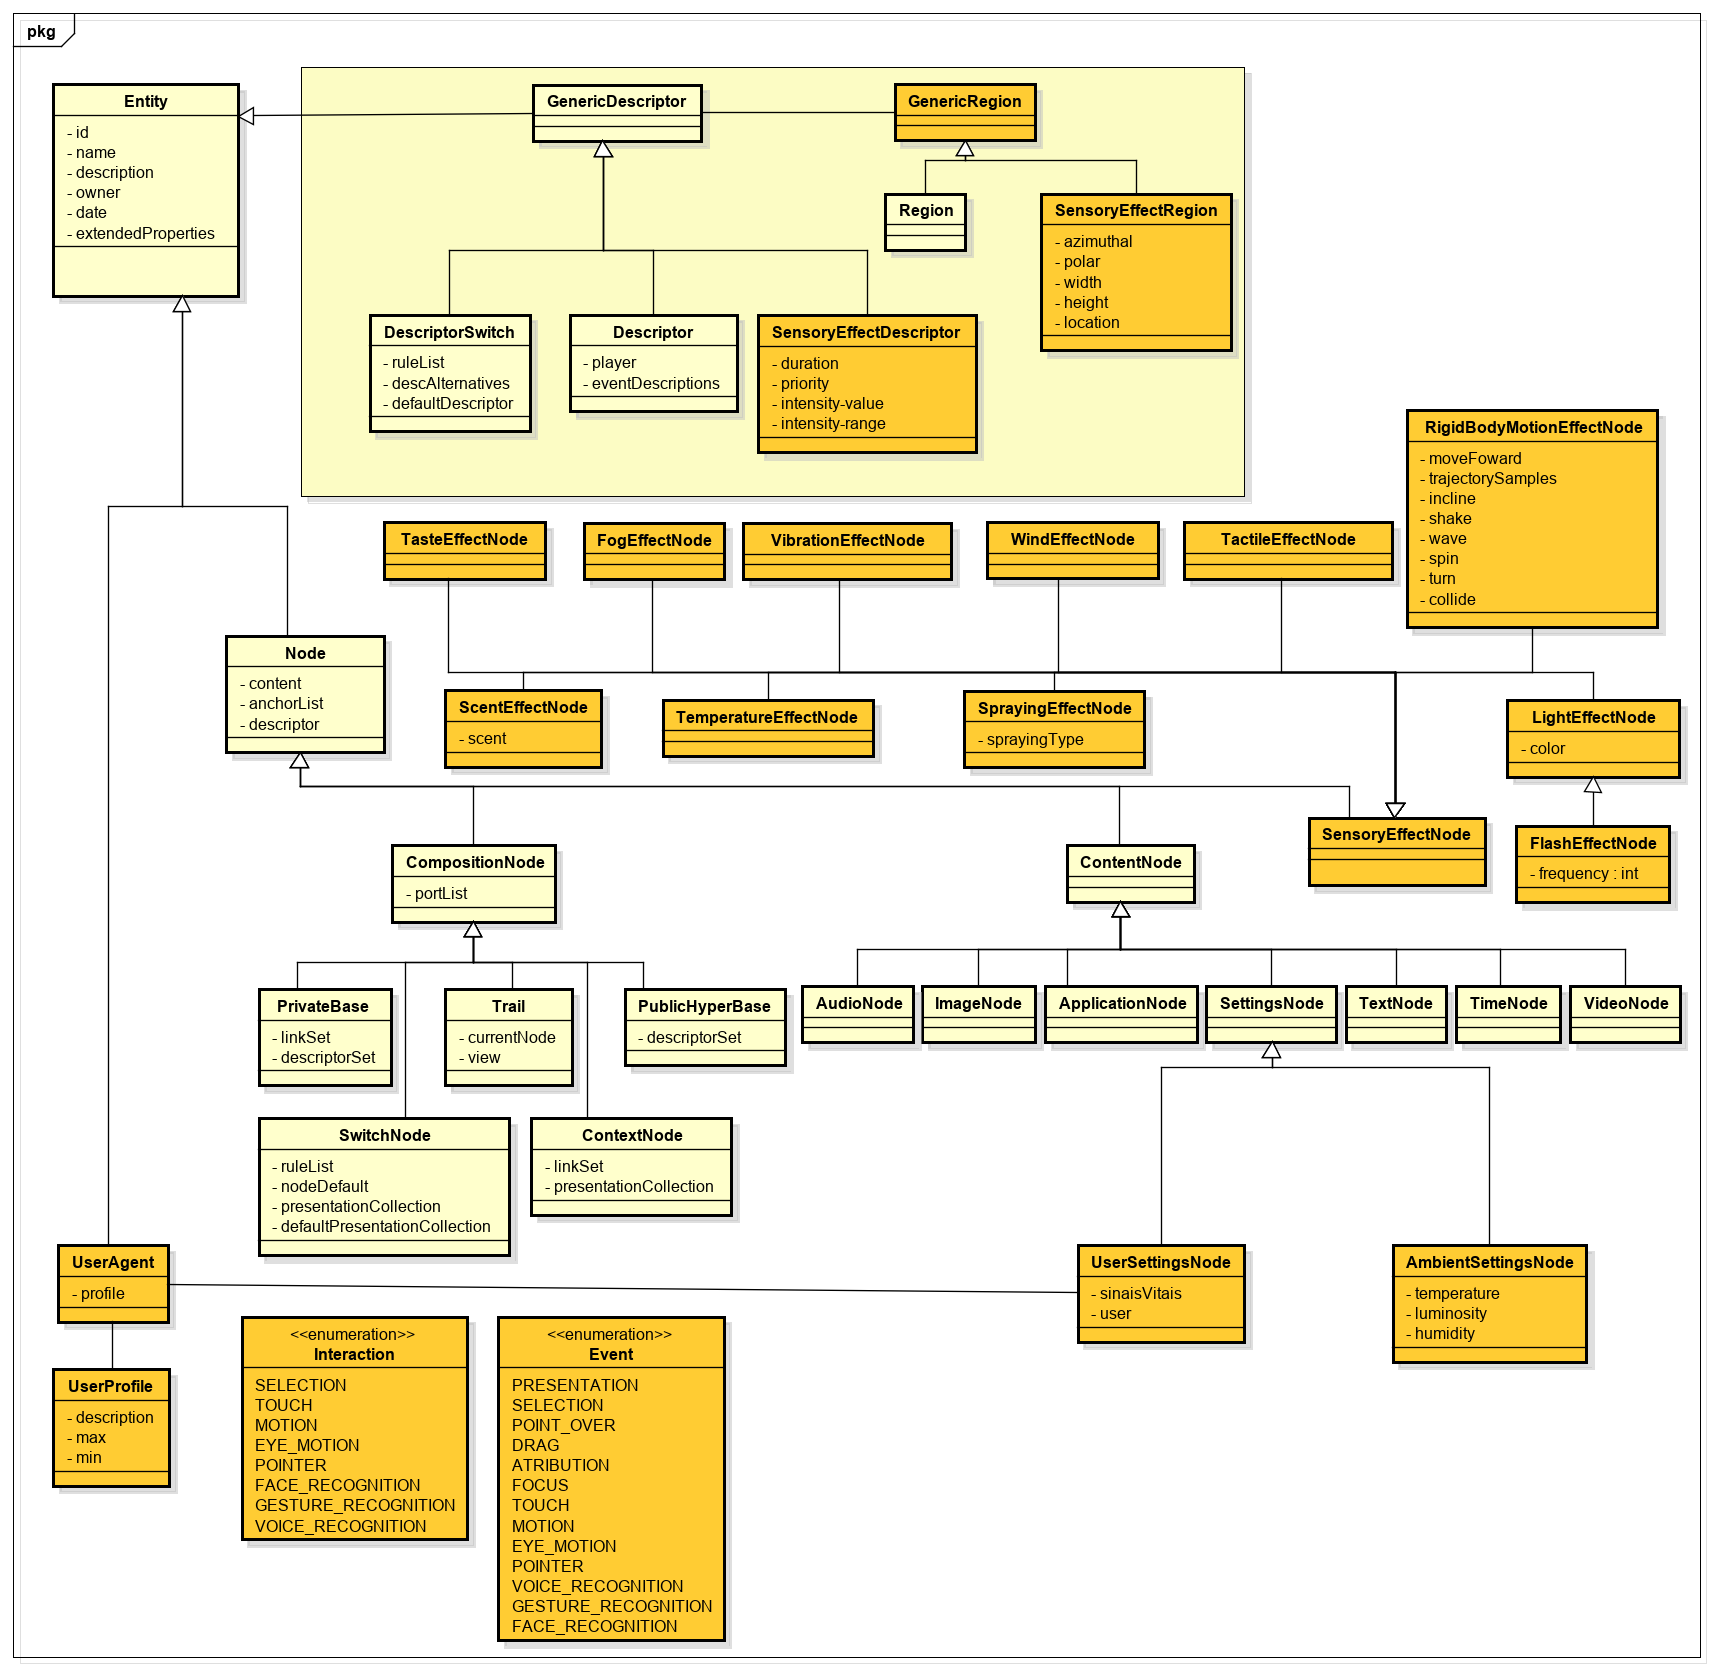
\includegraphics[scale=0.35,keepaspectratio=true]{figuras/NCM.png}
    \caption{Modelo NCM estendido.}
    \label{fig:NCMExt}
\end{figure}
%\end{landscape}

A Figura~\ref{fig:NCMExt}  apresenta o modelo NCM estendido conforme as propostas desta tese. As cores da figura ajudam a identificar o escopo deste trabalho. As entidades em amarelo fazem parte do modelo NCM 3.0 já existente. As entidades de cor laranja estão sendo propostas por este trabalho. Pode-se observar as entidades \textit{UserSettingsNode} e \textit{AmbientSettingsNode} como subclasses da entidade \textit{SettingsNode}, portanto herdando todas suas características como foi dito anteriormente. Pode-se observar também as entidades \textit{UserAgent} e \textit{UserProfile}, ambas subclasses de \textit{Entity}, \textit{UserAgent} associada com \textit{UserProfile} e \textit{UserSettingsNode}. A cardinalidade da associação de \textit{UserAgent} com \textit{UserProfile} é de muitos pra muitos pois um usuário pode ter vários perfis como por exemplo ter um perfil de esportista e ser um professor. Desta forma, o nó de conteúdo (\textit{UserSettingsNode}) que armazena as informações desse usuário pode armazenar informações desses dois perfis. E obviamente um perfil pode estar associados a vários usuários. Já a associação de \textit{UserAgent} com \textit{UserSettingsNode} é de um pra um. A Figura~\ref{fig:NCMExt} inclui também as entidades relacionadas a efeitos sensoriais, que foram propostas em Josue et al.\cite{Josue:2018:MSE:3204949.3204967}.

Além da extensão do modelo NCM, apresentada na Figura~\ref{fig:NCMExt}, este trabalho propõe uma extensão da linguagem NCL de maneira que o autor consiga usar novas facilidades para representação de múltiplos usuários e diferentes eventos de interação em sua aplicação multimídia. A extensão da linguagem NCL é discutida na próxima seção.

\section{NCL 4.0}

Para implementar as alterações no modelo NCM descritas na Seção~\ref{sec:NCMExt}, esta tese e os trabalhos \cite{barreto2019authoring,montevecchi2020providing,valentim2020possibilitando,Josue:2018:MSE:3204949.3204967, barreto2019ncl_u, barreto2019providing_MU,barreto2019providing} propõem uma extensão da linguagem NCL (\textit{Nested Context Language}) denominada NCL 4.0. Diversas alterações são sugeridas para expressar as entidades idealizadas na extensão do modelo proposta neste trabalho. A proposta de NCL 4.0 
é especificada utilizando \textit{XML schema} \cite{thompson2004xml}. O esquema proposto foi estendido do esquema da linguagem NCL 3.0\footnote{http://www.ncl.org.br/pt-br/schemasxml}. A extensão proposta contém os novos elementos além de alterações nos elementos existentes para contemplar o que foi modelado\footnote{https://github.com/FabioBarr/NCL4.0.git}.

A linguagem NCL 4.0 é divida em módulos e estes são agrupados em área funcionais. 



 
Esta tese foca nas entidades relacionadas com interação multimodal e multiusuário em aplicações multimídia. Para isso, propõe alteração no módulo \textit{Media} da área funcional \textit{Components}, onde foi modificado o elemento \textit{media} acrescentando mais dois tipos possíveis de nós \textit{settings}. Os novos eventos de interação foram contemplados com a alteração do módulo \textit{CausalConnectorFunctionality} da área funcional \textit{Connectors} com adição de novos tipos de evento e também novos papeis de condição predefinidos. Finalmente foi acrescentada uma nova área funcional denominada \textit{Users}, contendo o módulo \textit{User}, que define  os elementos \textit{userAgent} e \textit{userProfile}. 
 
A representação das entidades \textit{UserAgent} e \textit{UserProfile} é feita pela adição dos elementos XML  \textit{<userAgent>} e \textit{<userProfile>}. Tais elementos são definidos para representar um perfil ou um usuário individualmente. O elemento \textit{<userAgent>} possibilita ao autor criar uma aplicação sob medida com a representação de um usuário individualmente. A Tabela~\ref{tab:atUserAgent} apresenta seus atributos. Em \textit{src} é especificado o arquivo XML com as características do usuário seguindo o formato MEPG 21 parte 22 \cite{ISO/IEC:2019aa} e que serão carregadas para o nó \textit{userSettings} correspondente. Desta forma, o autor poderá criar links associados a essas propriedades. Além disso, os eventos de interação pode ser condicionados a usuários especificados com a cláusula <userAgent>.  A Listagem~\ref{lst:userAgent} apresenta um exemplo da definição de um usuário específico em NCL 4.0.

\begin{table}[h]
\caption{Descrição dos atributos do elemento <userAgent>}
\label{tab:atUserAgent}
\centering
{
  % distancia entre a linha e o texto
  \renewcommand\arraystretch{1.25}
  \begin{tabular}{|p{1,5cm}|p{4,5cm}|p{5cm}|p{3cm}|} \hline
   \multicolumn{1}{|c|}{Atributo} & \multicolumn{1}{|c|}{Descrição} & \multicolumn{1}{c|}{Valor} & \multicolumn{1}{c|}{Obrigatoriedade} \\ \hline 
    \textit{id} & Identifica o elemento dentro da aplicação NCL. & Qualquer cadeia de caracteres que comece com uma letra ou um sublinhado ("\_") e que contenha apenas letras, dígitos, "." e "\_". & Obrigatório \\  \hline
    \textit{src} & Define a URI do arquivo com as propriedades do usuário que serão carregadas. & Qualquer cadeia de caracteres que comece com uma letra ou um sublinhado ("\_") e que contenha apenas letras, dígitos, "." e "\_". & Opcional \\  \hline
  \end{tabular}
}
\end{table}

\begin{lstlisting}[language=ncl,label=lst:userAgent, caption={Definição de características de mais de um usuário de perfil diferente participante da aplicação}]
<userBase>
  <userAgent id="userA" src="user1.xml"/>
</userBase>
\end{lstlisting}

Outra maneira de representar os usuários é por meio do elemento \textit{<userProfile>}, da mesma forma que \textit{<userAgent>}, o perfil também tem o atributo \textit{src} que indica o caminho para o arquivo com as propriedades do perfil. Porém, neste caso as propriedades do perfil serão utilizadas para verificar se os usuários encontrado no \textit{setbox} (especificados por arquivos XML, por exemplo) correspondem as propriedades definidas no perfil. Caso haja, as propriedades dos usuários serão carregadas em nós do tipo \textit{userSettingsNode} correspondente. Assim os usuários que atendam ao perfil terão suas  propriedades consideradas pela aplicação. Além disso, para cada link criado com o perfil no parâmetro \textit{user}, serão criados links dinâmicos para todos que atendem o perfil. Tais links terão a identificação do usuário que foi especificada no arquivo de propriedades. A Tabela~\ref{tab:atUserProfile} apresenta os atributos do elemento \textit{<userProfile>} e a Listagem~\ref{lst:userProfile} apresenta um exemplo da definição de um perfil de usuário.  

\begin{table}[h]
\caption{Descrição dos atributos do elemento <userProfile>}
\label{tab:atUserProfile}
\centering
{
  % distancia entre a linha e o texto
  \renewcommand\arraystretch{1.25}
  \begin{tabular}{|p{1,5cm}|p{4,5cm}|p{5cm}|p{3cm}|} \hline
   \multicolumn{1}{|c|}{Atributo} & \multicolumn{1}{|c|}{Descrição} & \multicolumn{1}{c|}{Valor} & \multicolumn{1}{c|}{Obrigatoriedade} \\ \hline 
    \textit{id} & Identifica o elemento dentro da aplicação NCL. & Qualquer cadeia de caracteres que comece com uma letra ou um sublinhado ("\_") e que contenha apenas letras, dígitos, "." e "\_". & Obrigatório \\  \hline
    \textit{src} & Define a URI do arquivo com as propriedades do perfil de usuário. & Qualquer cadeia de caracteres que comece com uma letra ou um sublinhado ("\_") e que contenha apenas letras, dígitos, "." e "\_". & Obrigatório \\  \hline
    \textit{min} & Define o número mínimo de usuários que podem seguir este perfil na aplicação NCL. & número inteiro maior ou igual a zero (valor default é zero) & Opcional \\  \hline
    \textit{max} & Define o número máximo de usuários que podem seguir este perfil na aplicação NCL. & número inteiro maior ou igual ao valor do atributo min ou ``unbounded'' (valor default é ``unbounded'') & Opcional \\  \hline
  \end{tabular}
}
\end{table}


\begin{lstlisting}[language=ncl,label=lst:userProfile, caption={Definição de características de mais de um usuário de perfil diferente participante da aplicação}]
<userBase>
  <userProfile id="profile1" max="1" src="profile1.xml"/>
</userBase>
\end{lstlisting}

E finalmente outra possibilidade de se ter a participação do usuário identificada é sem a utilização do \textit{<userAgent>} e \textit{<userProfile>}. Basta colocar a palavra \textit{"all"} no parâmetro \textit{user} dos links construídos que da mesma forma do perfil, serão criados links dinâmicos para todos os usuários encontrados no \textit{setbox} sem fazer a validação do perfil.  Nós do tipo \textit{userSettingsNode} com valor \textit{"all"} resultarão em criação de nós dinamicamente.

As entidades \textit{UserSettingsNode} e \textit{AmbientSettingsNode} são expressas por meio de modificações no elemento \textit{<media>} onde foram adicionados dois novos tipos, um para representar características do usuário e outro para representar características do ambiente. Tais características podem ser estáticas lidas de arquivos ou dinâmicas lidas de sensores presentes no ambiente e/ou no usuário. Porém a linguagem NCL 3.0 não dá suporte a isso, pois conforme apresentado na norma ABNT NBR15606-2 \cite{ABNT:2011aa}, é permitido o armazenamento de variáveis em NCL 3.0 por meio de um nó <media> do tipo \textit{application/x-ncl-settings}. Estas podem ser globais definidas pelo autor ou de ambiente reservadas para o sistema Ginga. Alguns valores de propriedades do nó do tipo \textit{application/x-ncl-settings} podem ser modificadas através do uso de elos NCL.  Porém, só é permitido um nó do tipo ncl-settings em cada documento NCL. Neste contexto, este trabalho propõe adicionar mais dois tipos de mídia: "\textit{ambient-settings}" e "\textit{user-settings}" que  armazenam informações do ambiente e do usuário respectivamente. Estes com a cardinalidade maior que 1 como os outros tipos de nó \textit{<media>}, além de suas informações poderem ser advindas de sensores que deverão atualizar estes dados periodicamente ou definidos pelo autor do documento NCL. O nó <media> do tipo \textit{ambient-settings} (\textit{application/x-ncl-ambient-settings}) poderá usar a propriedade \textit{descriptor} para especificar um descritor que contém características de leitura das informações dos sensores como por exemplo, frequência de captura. A frequência de leitura indica a cada quanto tempo a mídia será atualizada com dados lidos do sensor.
Um elemento \textit{descriptor} associado a um nó \textit{ambient-settings} pode referenciar o elemento \textit{region} na qual define a região de captura de dados. A maneira com os sensores do ambiente vão ser ligados aos nós de ambiente pode ser definida através de um arquivo de configuração, que será definido no Capítulo~\ref{cap:cap5}.

A Listagem~\ref{lst:ambientSettings} apresenta um exemplo da utilização de \textit{ambient-settings}. O nó com id \textit{propLumRoom} descreve variáveis que irão armazenar características do ambiente, neste caso luminosidade e temperatura. Este nó contém uma propriedade para cada característica.

\begin{lstlisting}[language=ncl,label=lst:ambientSettings, caption={Definição de \textit{AmbientSettingsNode}}]
 <media type="application/x-ncl-ambient-settings" id="propLumRoom" >
   <property name="luminosity" />
   <property name="temperature" />
 </media>
\end{lstlisting}

O nó <media> do tipo \textit{user-settings} (\textit{application/x-ncl-user-settings}) funciona de maneira semelhante ao \textit{ambient-settings}.  A principal diferença é que os sensores não estão associados a um ambiente, mas sim a um usuário especificamente. Além de poder armazenar também características estáticas vindas de arquivos armazenados localmente ou repositórios pré-definidos. Tal arquitetura será definida no Capítulo~\ref{cap:cap5}. Para realizar a associação de sensores a um usuário, deve-se associar a mídia \textit{user-settings} a um \textit{id} de usuário. A Listagem~\ref{lst:ncl_userSettings} apresenta um exemplo da utilização de \textit{user-settings}. Pode ser observado que o \textit{user-settings} do exemplo está associado ao \textit{id} do usuário \textit{userB} definido na Listagem~\ref{lst:ncl_user}. Desta forma, todas as características contidas no XML poderão ser carregadas para o \textit{userSettingsNode} associado a um \textit{userAgent}.

\begin{lstlisting}[language=ncl,label=lst:ncl_userSettings, caption={Definição de \textit{UserSettingsNode}}]
  <media type="application/x-ncl-user-settings" id="propUserB" user="userB">
    <property name="heartBeat" />
    <property name="face" />
  </media>
\end{lstlisting}

Em NCL, utilizando conectores, relacionamentos de interação do usuário podem ser definidos \cite{soares2009programando}. E a definição de um conector é feita por um conjunto de papéis que determinam a função dos participantes da relação. Cada papel descreve um evento associado a um participante da relação. Os eventos de interação possuem o atributo \textit{key} que especifica o que foi reconhecido na interação do usuário. Na linguagem NCL, a interação multimodal é expressa com adição de eventos e novos papéis com os valores possíveis para o atributo \textit{key}. Essa adição de eventos, através dos papeis, segue o que foi modelado no Capítulo XXX representado na Figura~\ref{fig:NCMExt}. Para facilitar o uso desses novos eventos em NCL, são adicionados novos nomes reservados de papéis para o elemento  \textit{<simpleCondition>}. A Tabela~\ref{tab:papModal} apresenta os papeis relacionados a eventos de interatividade multimodal assim como os possíveis valores para o atributo \textit{key} propostos nesta tese.

\begin{table}[h]
\caption{Papeis propostos para contemplar as interações multimodais}
\label{tab:papModal}
\centering
{
  % distancia entre a linha e o texto
  \renewcommand\arraystretch{1.25}
  \begin{tabular}{|p{4,5cm}|p{6,5cm}|p{3,5cm}|} \hline
   \multicolumn{1}{|c|}{Papel} & \multicolumn{1}{|c|}{Descrição} & \multicolumn{1}{c|}{Atributo key}  \\ \hline 
  
    onVoiceRecognition & Quando algo dito pelo usuário for reconhecido enquanto o objeto associado a esse papel estiver sendo apresentado ou com foco. & trecho de voz reconhecido \\  \hline

    onFaceRecognition & Quando alguma expressão facial do usuário for reconhecida enquanto o objeto associado a esse papel estiver sendo apresentado ou com foco. & tipo da expressão facial do usuário \\ \hline

    onHandPoseRecognition & Quando algum gesto feito pelo usuário for reconhecido enquanto o objeto associado a esse papel estiver sendo apresentado ou com foco. & tipo do gesto do usuário \\  \hline

    onEyeGaze & Quando o usuário fixar o olhar em um região enquanto o objeto associado a esse papel estiver sendo apresentado ou com foco. & id do objeto que esta na região "olhada" \\  \hline

    onMotion & Quando algum movimento corporal feito pelo usuário for reconhecido enquanto o objeto associado a esse papel estiver sendo apresentado ou com foco. & tipo do movimento do corpo do usuário \\  \hline
    
    onTouch & Quando alguma interação por toque feita pelo usuário for reconhecida enquanto o objeto associado a esse papel estiver sendo apresentado ou com foco. & tipo do toque  \\  \hline
    
    onPointer & Quando um apontamento realizado pelo usuário for reconhecido enquanto o objeto associado a esse papel estiver sendo apresentado ou com foco. & posição do apontamento \\  \hline

  \end{tabular}
}
\end{table}

Conforme o trabalho de \cite{Josue:2018:MSE:3204949.3204967}, NCL 4.0 contém um novo módulo chamado \textit{Effect} dentro da área funcional \textit{Components}, que define o elemento \textit{effect} e seus atributos. Consequentemente os módulos \textit{Layout} e \textit{Descriptor} foram alterados. Mais especificamente, o \textit{Layout} foi alterado ao acrescentar atributos ao elemento \textit{region} e \textit{Descriptor} foi alterado ao acrescentar atributos ao elemento \textit{descriptor}. As entidades NCM do tipo \textit{SensoryEffectNode} são implementadas através do elemento \textit{<effect>} em NCL 4.0, junto com seus atributos \textit{id}, \textit{type} e \textit{descriptor}. Tais atributos vão identificar, especificar e descrever as características da ocorrência do efeito sensorial. A propriedade \textit{type} será descrita seguindo a nomenclatura de tipos de efeitos sensoriais definidos no padrão MPEG-V \cite{yoon2015mpeg}. Em Josue et al.\cite{Josue:2018:MSE:3204949.3204967}, há uma discussão aprofundada sobre a implementação e descrição de elementos que integram efeitos sensoriais em uma aplicação multimídia imersiva. %E a implementação dos efeitos sensoriais por meio da linguagem NCL 4.0 é descrita em \cite{barreto2019authoring}.


Este capítulo apresentou a propostas de extensão tanto do modelo NCM quanto da linguagem NCL. Essas propostas foram consolidadas em uma nova versão da linguagem NCL, chamada NCL 4.0. Para isso, o capítulo detalhou as novas entidades que fazem parte da extensão assim como as alterações que abrangem o modelo e a linguagem. O capítulo apresentou as duas principais contribuições desta tese em seções que falam sobre multiusuário, informações de contexto e multimodalidade. NCL 4.0 reúne facilidades para especificação de aplicações  multissensoriais interativas e multiusuário, possibilitando a evolução da TV digital interativa para TV imersiva multimodal e multiusuário.

O próximo capítulo apresenta a  implementação de NCL 4.0 no \textit{middleware} Ginga-NCL de todos os elementos propostos assim como alterações necessárias para que o Ginga-NCL contemple a proposta. Desta forma, possibilitando a implementação e a execução de aplicações NCL 4.0 com as funcionalidades citadas.
\chapter{Implementação no Middleware Ginga-NCL} \label{cap:cap5}

O Ginga-NCL é o subsistema do \textit{middleware} Ginga, padrão do Sistema Brasileiro de TV Digital, que permite a execução de aplicações multimídia especificadas na linguagem NCL \cite{ABNT:2011aa}. Atualmente, o subsistema dá suporte apenas a interações de um usuário por meio do controle remoto ou mouse. Visando dar suporte a outras modalidades de interação, suporte multiusuário e armazenamento de informações contextualizadas por usuários (ou grupo de usuários) nas aplicações, esta tese propõe a inclusão de novos componentes no \textit{middleware}\footnote{A implementação de extensão do Ginga-NCL apresentada neste trabalho pode ser acessada em  bit.do/gingaMultimodalBranch.}, conforme será detalhado nas seções a seguir. %mostra a Figura \ref{fig:arquitetura}. 
Para o desenvolvimento da proposta foi utilizada a implementação de referência da máquina de apresentação\footnote{https://github.com/TeleMidia/ginga} do Ginga-NCL. A Figura \ref{fig:arquitetura} ilustra a arquitetura da implementação estendida do \textit{middleware} Ginga-NCL.

\begin{figure}[h!]
    \centering
    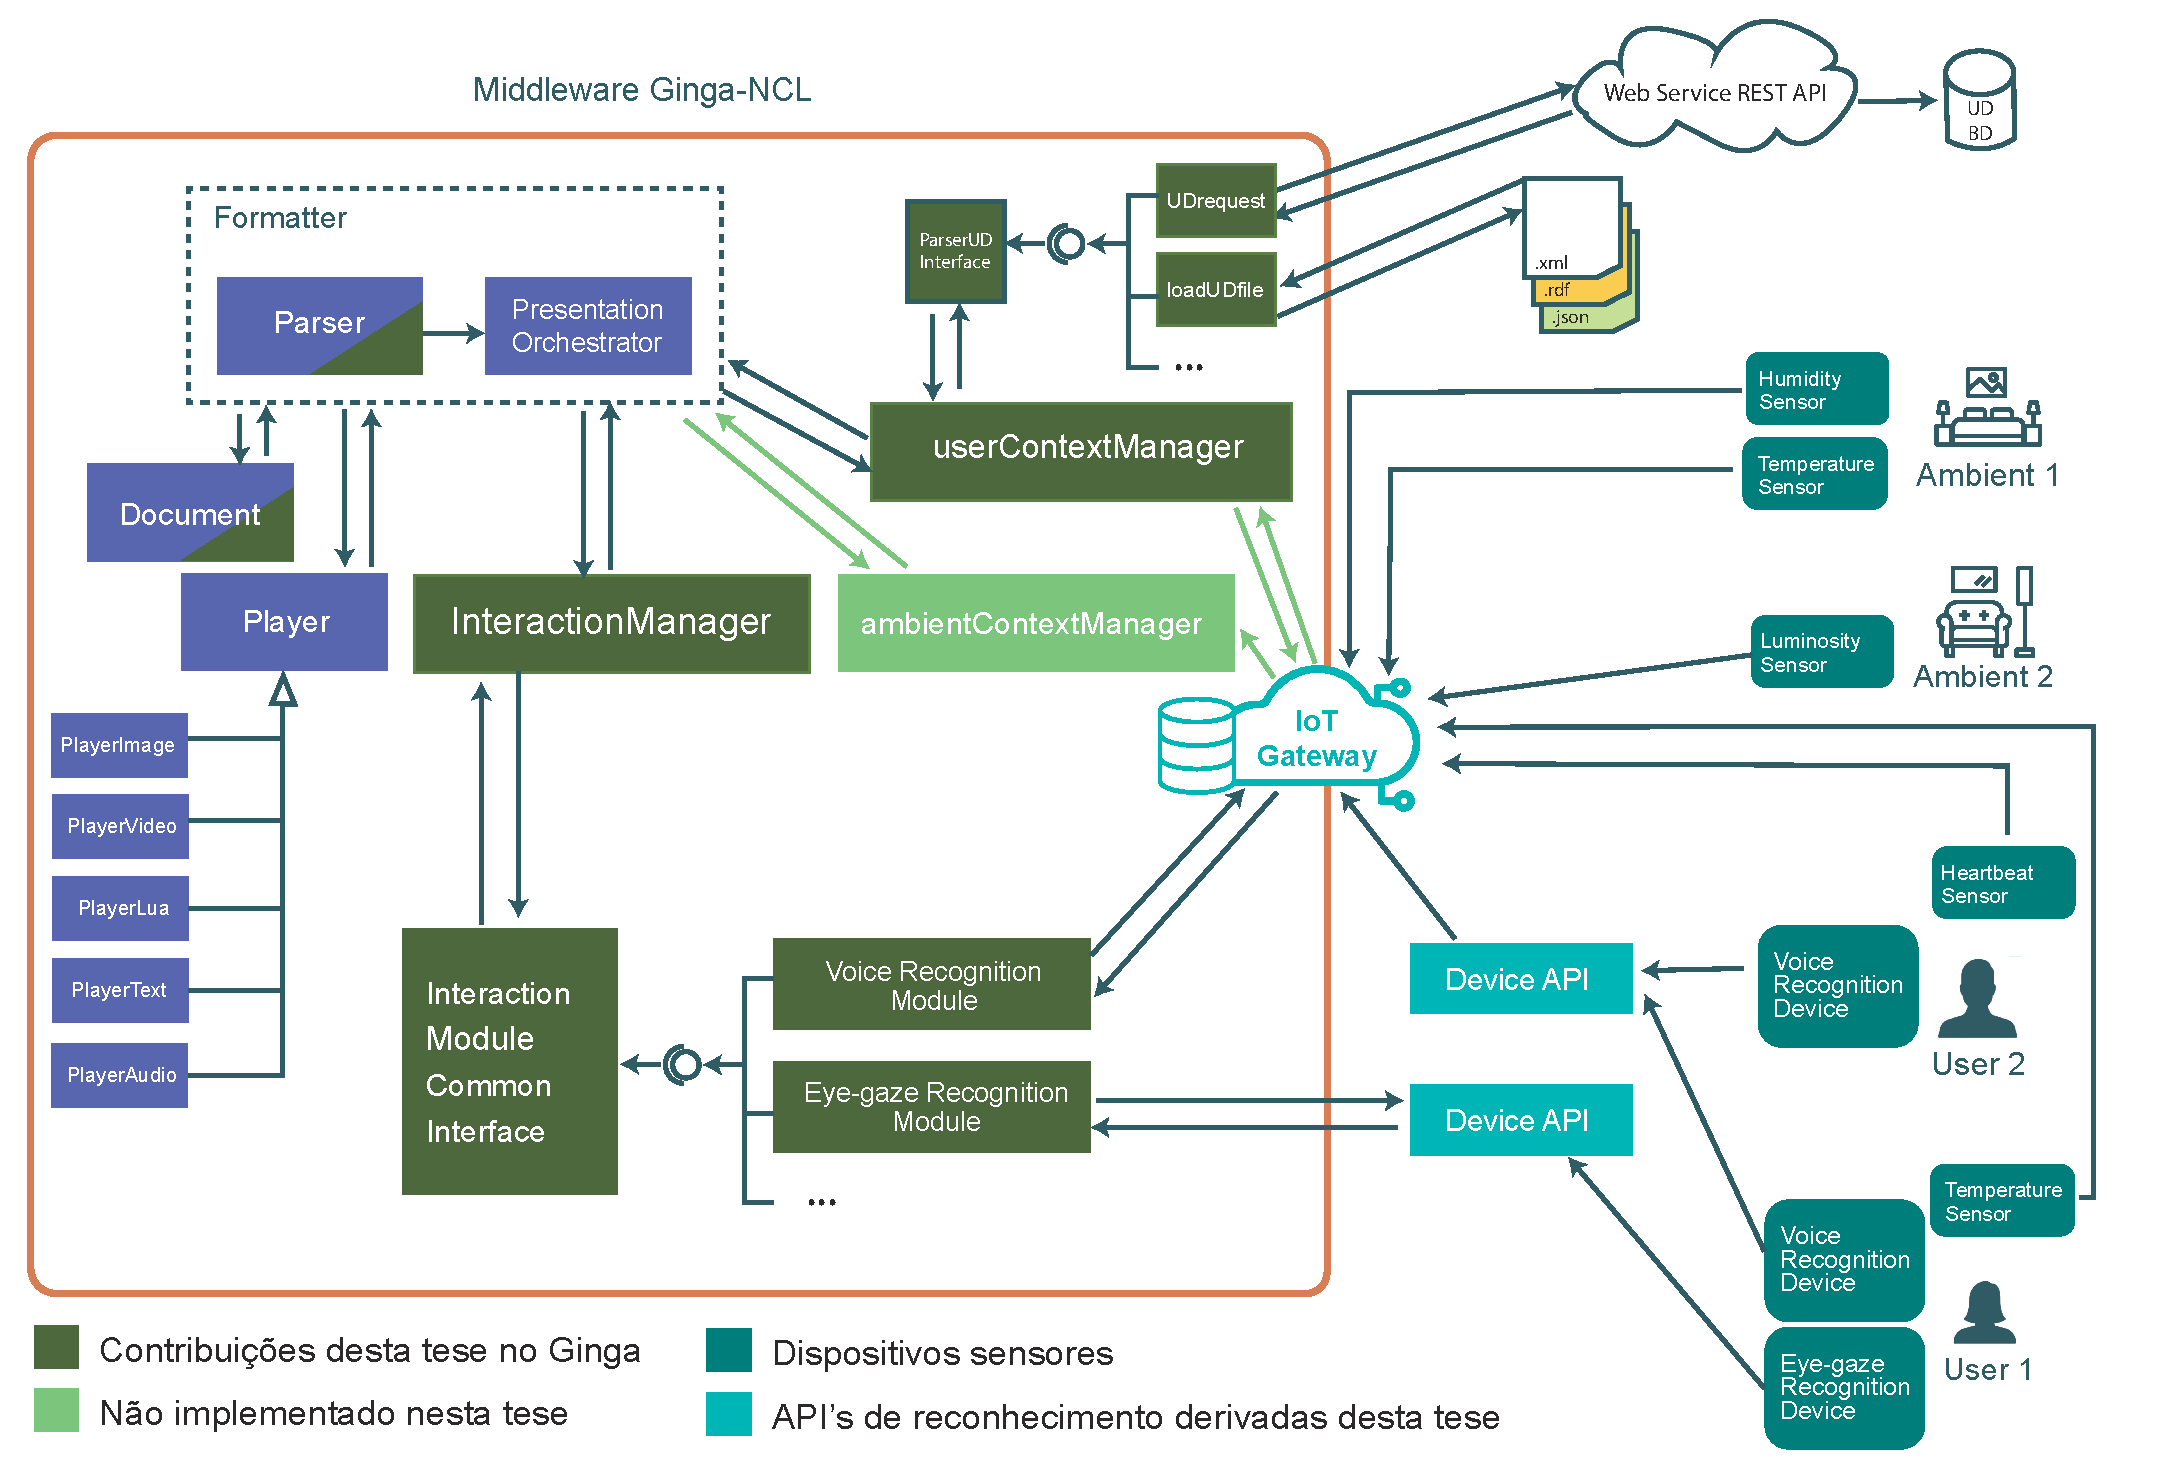
\includegraphics[scale=0.43, keepaspectratio=true]{figuras/ArqPropExt.pdf}
    \caption{Arquitetura estendida do Ginga-NCL para suporte à interação multimodal com múltiplos usuários.}
    \label{fig:arquitetura}
\end{figure}

\section{Interação multimodal e multiusuário}

O componente \textit{Formatter}, presente na atual versão do Ginga, é o responsável por controlar a apresentação dos objetos de mídia que compõem uma aplicação. Além disso, este elemento manipula os eventos de interação do usuário com a aplicação. Ao iniciar uma aplicação multimídia, o \textit{Formatter} envia o documento NCL para o \textit{Parser}, que extrai as informações sobre os elementos que compõem a aplicação e as relações de sincronização espaço-temporal definidas pelo autor da aplicação multimídia. 

O controle das interações do usuário com a aplicação multimídia é realizado pelo componente \textit{InteractionManager} proposto neste trabalho. É por meio do \textit{InteractionManager} que os dispositivos de interação se comunicam com o \textit{Formatter}, notificando-o quando ocorre uma interação por parte do usuário. O \textit{InteractionManager} ativa os diferentes módulos de interação, conforme especificado pelo documento NCL, e passa, para cada um deles, as informações sobre o que deve ser monitorado durante a execução da aplicação. A fim de permitir que a implementação seja facilmente estendida para adição de novas modalidades de interação, foi criada uma interface (\textit{Interaction Module Common Interface}), que deve ser implementada por cada módulo de interação específico. Note que, se a aplicação não utiliza um determinado tipo de interação, o módulo correspondente não será iniciado pelo \textit{InteractionManager} desnecessariamente.

Para a implementação da interação multimodal proposta nesta tese, os componentes \textit{Parser} e \textit{Formatter} foram estendidos, para dar suporte ao reconhecimento de novos tipos de eventos definidos em NCL 4.0 e  detalhados no Capítulo~\ref{cap:cap4}. Se elos da aplicação NCL associam eventos de interação a usuários ou perfis específicos, na fase de análise do documento, o \textit{Parser} faz o mapeamento entre a interação e o usuário associado a ela, por meio da análise dos elementos \textit{<link>} especificados. Por exemplo, ao analisar o elo definido na Listagem \ref{lst:ncl_multmodal}, o \textit{Parser} irá informar ao \textit{Formatter} que é preciso ativar o módulo responsável pelo reconhecimento de voz~(\textit{Voice Recognition Module}), além de enviar para esse módulo o usuário "\textit{user1}" (atributo \textit{user}) e palavra chave  "\textit{play}" (atributo \textit{key}) relacionados à interação e que ele deve notificar ao reconhecedor. Essa notificação é feita ao módulo \textit{InteractionManager}.

\begin{lstlisting}[language=ncl,label=lst:ncl_multmodal, caption={Conector e elo para interação mutimodal em NCL estendido}]

...
<connectorBase>
   <causalConnector id="onVoiceRecognitionStart">
      <connectorParam name="key"/>
      <connectorParam name="user"/>      
      <simpleCondition role="onVoiceRecognition" key="$\$$key" user= "$\$$user"/>
      <simpleAction role="start" />
   </causalConnector>  
</connectorBase>
...
<link xconnector="onVoiceRecognitionStart">
 	<bind role="onVoiceRecognition" component="botanicalGardenImage">
  		<bindParam name="key" value="play"/>
   		<bindParam name="user" value="user1"/>
 	</bind>
 	<bind role="start" component="botanicalGardenVideo"/>
 </link> 
...
\end{lstlisting}

%O controle das interações do usuário com a aplicação multimídia é realizado pelo componente \textit{InteractionManager} proposto neste trabalho. É por meio do \textit{InteractionManager} que os dispositivos de interação se comunicam com o \textit{Formatter}, notificando-o quando ocorre uma interação por parte do usuário. O \textit{InteractionManager} ativa os diferentes módulos de interação, conforme especificado pelo documento NCL, e passa, para cada um deles, as informações sobre o que deve ser monitorado durante a execução da aplicação. A fim de permitir que a implementação seja facilmente estendida para adição de novas modalidades de interação, foi criada uma interface (\textit{Interaction Module Common Interface}), que deve ser implementada por cada módulo de interação específico. Note que, se a aplicação não utiliza um determinado tipo de interação, o módulo correspondente não será iniciado pelo \textit{InteractionManager} desnecessariamente.

Os módulos de interação e o \textit{InteractionManager} se comunicam através de métodos pré-definidos pela interface (\textit{Interaction Module Common Interface}). Por exemplo, o \textit{InteractionManager}, ao ativar um módulo de interação, envia um objeto JSON (\textit{JavaScript Object Notation}) com uma lista de \textit{keys} que devem ser monitoradas pelo módulo, e os usuários relacionados àquela interação. Esta lista de \textit{keys} enviada pelo \textit{InteractionManager} depende do tipo de interação. Por exemplo, para o \textit{Voice Recognition Module}, são enviadas palavras ou frases a serem reconhecidas, e para o \textit{Gesture Recognition Module}, os tipos de gestos utilizados na aplicação. A Listagem~\ref{lst:json-exemplo} mostra um exemplo de JSON que segue o modelo para mapeamento de reconhecimento de voz, que gera o evento definido no \textit{link} na Listagem~\ref{lst:ncl_multmodal}.

\begin{lstlisting}[language=ncl,label=lst:json-exemplo, caption={Exemplo de JSON que usa o modelo para mapeamento de reconhecimento de voz para a Listagem~\ref{lst:ncl_multmodal}.}]
 {
    "userKeyList": [
        {
            "user": "user1",
            "key": [ "play"]
        }
    ]
 }
\end{lstlisting}



Na arquitetura proposta ilustrada na Figura \ref{fig:arquitetura}, pode-se perceber que o trabalho de reconhecimento da interação não é feito pelo formatador, evitando assim uma sobrecarga de processamento. Ele é notificado pelo \textit{InteractionManager} apenas se ocorrer uma interação que deve ser tratada pela aplicação. Ou seja, em uma aplicação multimídia que especifica apenas interação por voz, tendo como \textit{key} a palavra "\textit{play}", caso o usuário diga quaisquer outras palavras diferentes, nenhuma notificação será enviada ao \textit{InteractionManager}, e consequentemente ao formatador. Além disso, quando um módulo de interação específico notifica uma interação, ele pode também informar qual o usuário que a realizou, que no exemplo seria o "user1". Dentre os métodos que os módulos de interação devem implementar estão: \textit{start()}, \textit{setUserKeyList(json)} e \textit{stop()}, que possibilita ao \textit{InteractionManager} iniciar, passar as informações (\textit{keys}) que devem ser reconhecidas e parar o módulo de interação. Estes métodos são virtuais na classe \textit{InteractionModule}, portanto para desenvolver um novo módulo de interação funcionando nesta arquitetura, é necessário estender a classe \textit{InteractionModule}. Exemplos de subclasses de \textit{InteractionModule} na Figura \ref{fig:arquitetura} são \textit{Eye-gaze Recognition Module} e \textit{Voice Recognition Module}. 

\subsection{Reconhecimento de Voz em Ginga-NCL}

Com objetivo de validar a solução proposta, esta seção apresenta a implementação do módulo \textit{VoiceRecognitionModule} no Ginga-NCL utilizando uma API de reconhecimento de voz. A implementação de \textit{VoiceRecognitionModule} no Ginga utiliza a interface de comunicação comum a todos os dispositivos de interação (\textit{Interaction Module Common Interface}). Nesta implementação, o dispositivo de reconhecimento de voz se comunica com o Ginga utilizando o protocolo MQTT \cite{hunkeler2008mqtt}. Para isso, foram usadas funções do \textit{Google Cloud} para suprir a necessidade da conversão \textit{speech-to-text} \cite{bijl2001speech}. Inicialmente, é necessária a aplicação \textit{Google Assistant} para captar a voz do usuário e uma \textit{Action} do Google. Uma \textit{Action} é, essencialmente, uma aplicação que roda sobre o \textit{Google Assistant}, estendendo suas funcionalidades. Como ilustrado pela Figura~\ref{fig:action}, para a \textit{Action} se comunicar com o broker MQTT, ela utiliza o serviço Google \textit{Firebase} para que seja feita a publicação MQTT. 

Em resumo, o \textit{VoiceRecognitionModule} se inscreve em um tópico MQTT criado para o módulo de reconhecimento de voz. Isso é feito na execução do método \textit{start()} e portanto a instância passa a ouvir publicações no tópico que a \textit{Action} usa. Assim, a API do Google publica uma mensagem nesse tópico, significando que o dispositivo reconheceu o que foi dito. Quando ocorre a publicação do texto reconhecido no broker MQTT, o \textit{VoiceRecognitionModule} compara seu conteúdo com a lista de \textit{keys} e \textit{users} de interesse da aplicação. Se for uma palavra ou frase associado a um usuário de interesse ao Ginga, notifica o \texttt{InteractionManager}, que por sua vez dispara o evento de reconhecimento de voz no formatador.

\begin{figure}[h!]
    \centering
    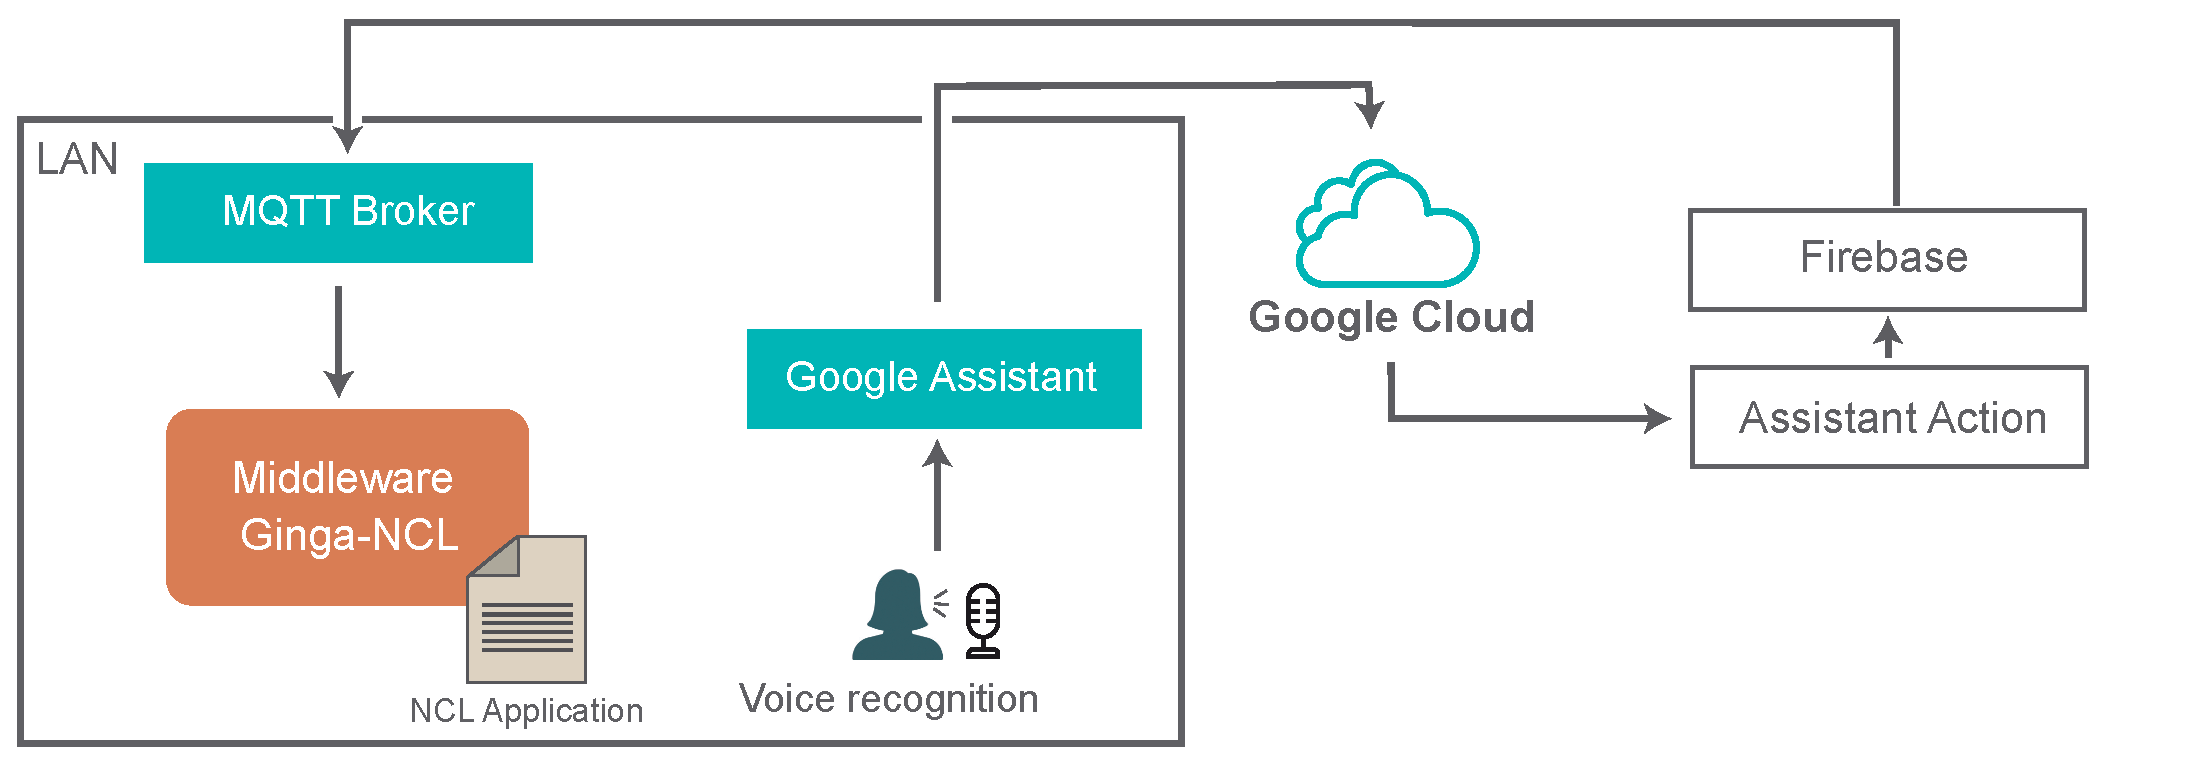
\includegraphics[scale=0.35, keepaspectratio=true]{figuras/arq-action-eng.pdf}
    \caption{Arquitetura do reconhecimento de voz na implementação atual.}
    \label{fig:action}
\end{figure}

A \textit{Action}, ao ser invocada, encaminha em forma de texto, todos comandos de voz que sejam precedidos por "TV". Desse modo, caso se queira executar na aplicação um comando denominado "iniciar", diz-se "TV iniciar". Há, ainda, uma configuração opcional de perfis de usuário. Ao dizer "Definir perfil como...", o que vier depois é vinculado ao dispositivo corrente como sendo o perfil ou a identificação daquele usuário. Feito isso, todos os comandos enviados à aplicação são precedidos por esse perfil ou identificação, relacionado ao usuário que interagiu.

A título de exemplo, em uma aplicação que contém um terapeuta e um paciente, de forma que cada perfil tem acesso a um conjunto de comandos diferentes, o usuário ao se identificar por terapeuta, em seu dispositivo, invoca "Definir perfil como terapeuta" e, analogamente, o paciente faz o mesmo. A partir disso, a aplicação será capaz de decidir, baseado nos perfis, quem invoca qual comando.

Outra implementação, seguindo a arquitetura da Figura~\ref{fig:arquitetura}, foi proposta em \cite{montevecchi2020providing}, onde sensores de rastreamento ocular permitem que os usuários interajam pelo olhar com aplicativos multimídia, proporcionando assim também uma nova modalidade de interação para as aplicações de TV digital. Em \cite{montevecchi2020providing}, foi proposta uma extensão Ginga-NCL para fornecer interação através de fixação do olhar usando um dispositivo rastreador de olhos e permitir o uso de um novo tipo de evento para autoria  em NCL, chamado \textit{EyeGaze}.

O trabalho de  \cite{valentim2020possibilitando} utiliza a  arquitetura proposta na Figura~\ref{fig:arquitetura} para possibilitar o reconhecimento de expressões faciais para que a TV que seja agnóstica à implementação do algoritmo de reconhecimento. Como prova de conceito, a  proposta do artigo foi desenvolvida sob o \textit{middleware} Ginga-NCL. Foram realizadas duas implementações: a primeira baseada na versão atual do \textit{middleware} Ginga e a segunda baseada em uma extensão proposta ao \textit{middleware}, mostrando a viabilidade da proposta apresentada.

\section{Suporte Multiusuário e Informações de Contexto}

A atual versão do \textit{middleware} Ginga-NCL captura as interações vindas de dispositivos como controle remoto, mouse ou teclado representando a interação de um usuário somente. Suas informações são armazenadas em um nó de conteúdo do tipo \textit{settingsNode} onde também são armazenadas informações gerais da aplicação NCL. Só é permitido um nó desse tipo por aplicação NCL. Algumas dessas propriedades não podem ser alteradas durante a execução da aplicação. Se mais de um usuário interage com a aplicação e essa precisa mudar seu comportamento de acordo com propriedades específicas de quem participa da experiência, não seria possível construir um documento NCL para atender a esse caso de uso na versão atual do Ginga-NCL.

O elemento XML <\textit{userAgent}> foi implementado por meio de uma estrutura \textit{user} que armazena propriedades de um usuário como um identificador e o caminho do arquivo onde estão suas informações individuais. Já o <\textit{userProfile}> foi implementado com a construção da estrutura \textit{profile} que mantém um identificador, numero mínimo e máximo de usuários que podem estar associados ao perfil e o caminho para as informações do perfil. A implementação mantém, no formatador, uma lista de estruturas do tipo \textit{user} e outra lista do tipo \textit{profile}. Desta forma, é possível ao formatador associar os \textit{links} de interação com os usuários ou perfis a estas listas; Carregar informações destes usuários para nós de conteúdo do tipo \textit{userSettingsNode} podendo também criar elos com esses nós. Finalmente pode-se associar a essa lista sensores, que podem coletar informações dos usuários participantes da experiência multimídia, como batimento cardíaco ou temperatura.

Os elos são associados ao usuário da maneira como foi descrita na Seção anterior, ou seja, o \textit{InteractionManager} envia para os módulos as listas de usuário que participam dos elos por meio de seu atributo \textit{user}. O valor do atributo \textit{user} deve fazer parte das listas de \textit{users} ou \textit{profiles} mantidas pelo formatador. Assim o autor da aplicação precisa definir o elemento  \textit{userAgent} e/ou \textit{userProfile} para poder referenciá-lo em elos com eventos de interação.

Conforme apresentado na Figura~\ref{fig:arquitetura}, o \textit{userContextManager} gerencia a importação das informações associadas tanto a \textit{userAgent} quanto a \textit{userProfile}. As informações podem estar dispostas em arquivos como por exemplo XML, RDF ou JSON ou ainda estarem disponíveis em um banco de dados remoto  acessado por meio de API REST. O caminho do arquivo ou a string de conexão fica armazenada no atributo \textit{src} do \textit{userAgent} ou \textit{userProfile}. O carregamento dessas informações é feito por um módulo que implementa a interface \textit{ParserUDInterface}, como por exemplo, \textit{UDRequest} e \textit{loadUDFile}. Este módulo irá carregar todas as informações presentes no arquivo ou no banco de dados de acordo com a fonte de cada um. Para que um novo formato de arquivo seja contemplado pelo \textit{userContextManager}, basta implementar um classe filha de \textit{ParserUDInterface}. O módulo \textit{userContextManager} irá passar aos "importadores" (módulos que implementam \textit{ParserUDInterface}) todos os dados necessários para importação e armazenamento das propriedades desses usuários ou perfis. 

As informações trazidas serão armazenadas em nós de conteúdo do tipo \textit{userSettingsNode} gerenciados pelo \textit{UserContextManager}. Esses nós são instâncias de \textit{userSettingsNode} associados aos elementos  <\textit{userAgent}> ou <\textit{userProfile}>. Como prova de conceito, foi desenvolvido o módulo \textit{loadUDFile} para  arquivos XML seguindo o padrão MPEG-21 parte 22. Este módulo vai preencher o objeto da classe \textit{UserSettingsNode} associado a instância do \textit{UserAgent} respectivo.  Se o \textit{UserAgent} estiver associado ao \textit{UserProfile}, além das informações individuais referenciadas no \textit{UserAgent}, também serão consideradas as informações associadas aos \textit{UserProfiles}. A partir do momento em que as informações estão em nós do tipo \textit{userSettingsNode}, poderão ser utilizadas em elos com eventos de atribuição NCL.

As instâncias de \textit{UserSettingsNode} podem ser usadas também para armazenar informações lidas de um sensor em um ambiente IoT. Como pode-se verificar na Figura~\ref{fig:arquitetura}, pode-se ter sensores (com por exemplo \textit{Heartbeat Sensor} no User2) publicando leituras em um servidor IoT e o \textit{userContextManager} pode ler essas publicações e atualizar os nós do tipo \textit{UserSettingsNode} respectivos. Para isso, o gerenciador de contexto deve ter um assinante de um tópico no servidor IoT. Tomando como exemplo a arquitetura MQTT, pode-se ter um \textit{broker} MQTT recebendo publicações dos sensores e o gerenciador de contexto pode se inscrever nos mesmos tópicos de publicações dos sensores e atualizar as propriedades respectivas nos nós de conteúdo do tipo \textit{userSettingsNode} a partir da atualização das propriedades. Elos poderão ser ativados mudando o comportamento da aplicação de acordo com leituras feitas pelos sensores. De maneira análoga, o mesmo pode ser feito com sensores de ambiente (como por exemplo \textit{LuminositySensor} no Ambient 2 na Figura~\ref{fig:arquitetura}), publicando suas leituras no servidor IoT. E o gerenciador de contexto de ambientes (\textit{ambientContextManager}) pode pegar essas informações e atualizar os nós do tipo \textit{ambientSettingsNode}. Como também são nós de conteúdo, a atualização de suas propriedades pode ativar elos e disparar ações na aplicação. A implementação do \textit{ambientContextManager} 
é trabalho futuro.

Além de ler as informações publicadas pelos sensores de um servidor IoT, O \textit{userContextManager} pode também publicar informações específicas para que o dispositivo IoT leia, como por exemplo, informações para calibragem do dispositivo. Assim o gerenciador pode-se comunicar com o servidor nos dois sentidos. A comunicação entre o \textit{userContextManager} e o servidor IoT também 
é trabalho futuro.

Falta ressaltar que a arquitetura é extensível a vários tipos de evento de interação, dispositivos e sensores.

Este capítulo apresentou a implementação da proposta desta tese no \textit{middleware} Ginga-NCL, incluindo uma arquitetura extensível seus módulos e funcionamento geral. O capítulo exemplificou aplicações NCL desenvolvidas e utilizadas nos testes de funcionalidades. Apresentou também o formato dos dados que são trocados entre os módulos, como por exemplo, objetos JSON. O próximo capítulo apresenta a avaliação da proposta por meio de comparação com a implementação padrão atual do Ginga-NCL e também testes de carga que atestam o desempenho do \textit{middleware}.
\chapter{Resultados} \label{cap:cap6}




\chapter{Casos de Uso} \label{cap:cap7}

Este capítulo apresenta alguns casos de uso onde as funcionalidades propostas nesta tese são pertinentes. 

\section{Multimodalidade} \label{sec:casoUsoMultimodalidade}

Esta seção apresenta casos de uso que explora deferentes modalidades de interação.

\subsection{Navegação multimodal}
A aplicação desenvolvida para ilustrar a combinação de modalidades diferentes de interação combina interação via voz e teclas do controle remoto. Ela possui três vídeos que poderão ser apresentados de acordo com o desejo do usuário. No primeiro momento, o usuário escolhe dentre três opções para exibir o primeiro vídeo. Selecionando um dos botões, o vídeo respectivo será apresentado. A interface inicial da aplicação é apresentada na Figura~\ref{fig:appMultmodal}. Após o início de qualquer um dos vídeos, o usuário poderá dizer ``trocar'' e então os botões com as opções aparecerão novamente possibilitando a troca do vídeo que está sendo apresentado. Ao selecionar outro vídeo, o atual será parado e o escolhido será exibido. A aplicação é apresentada na Listagem~\ref{lst:appIntMultModal}.

\begin{figure}[h!] 
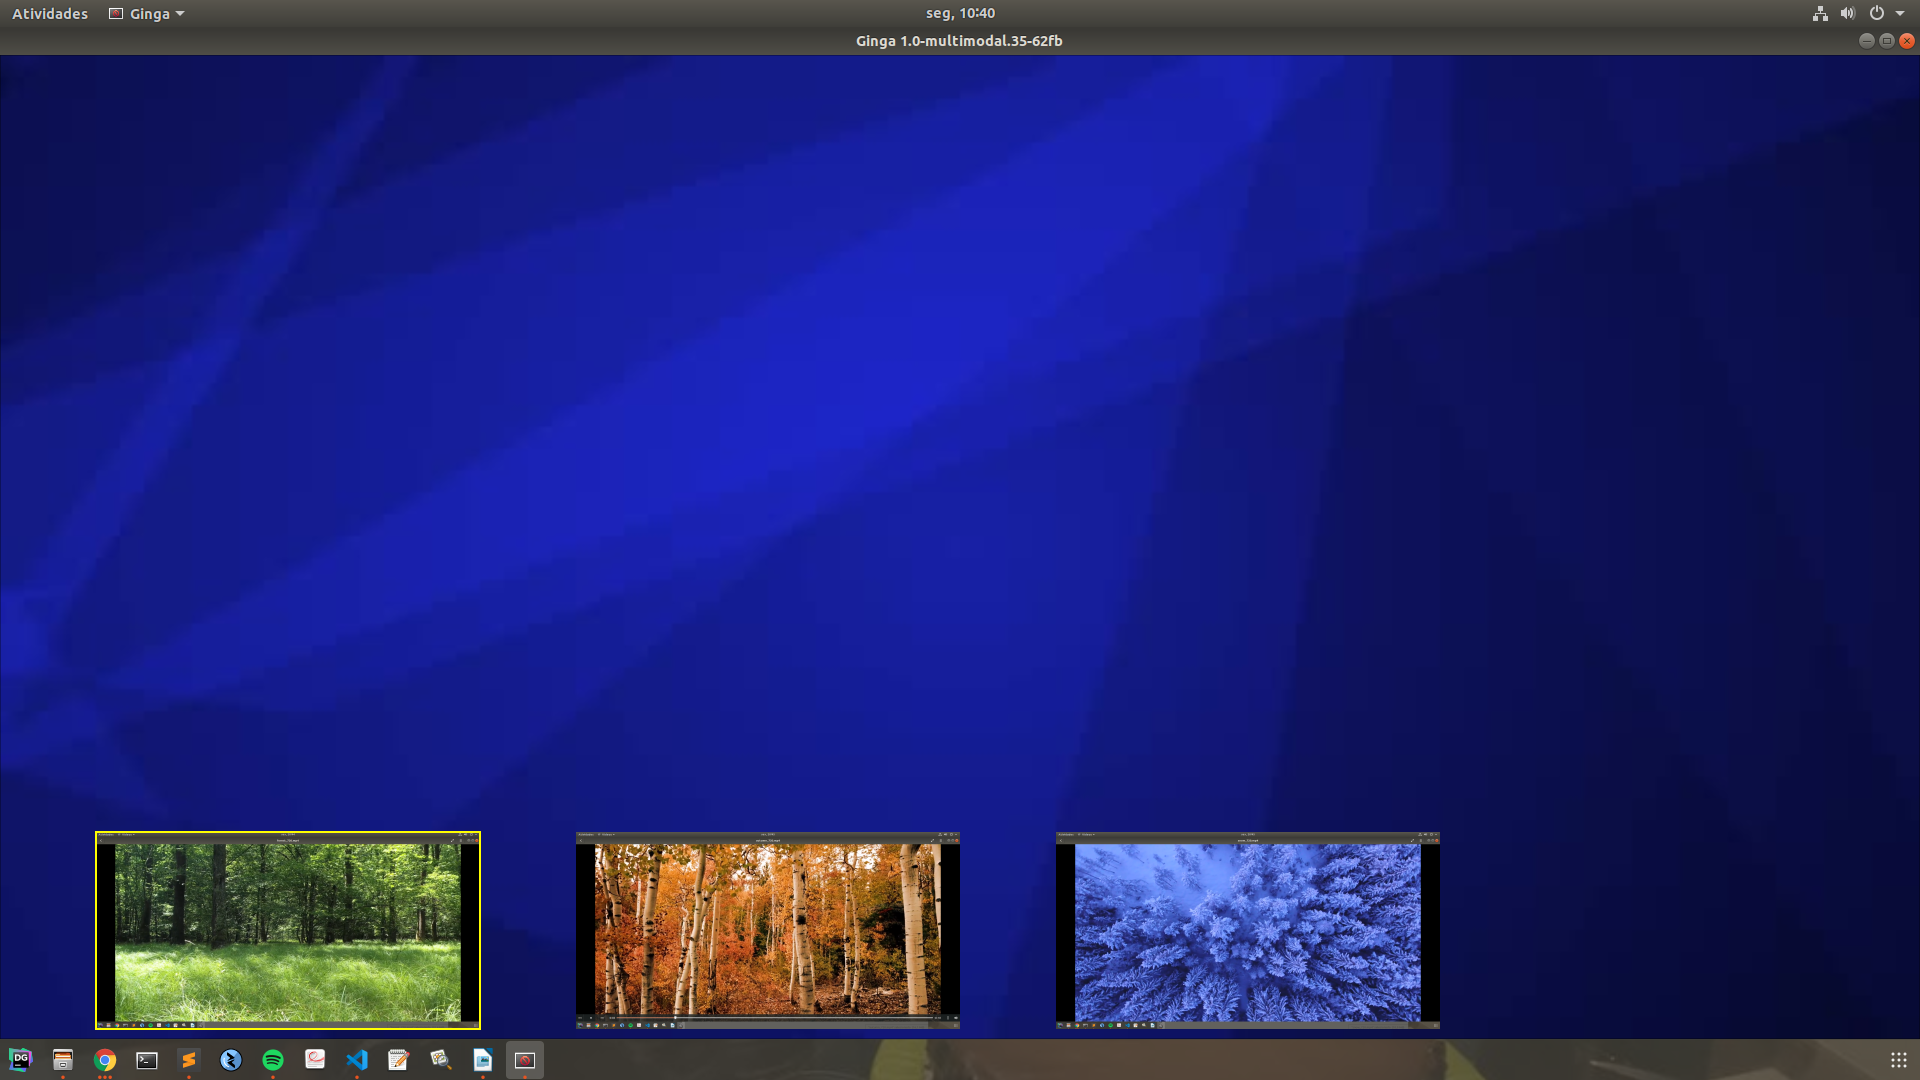
\includegraphics[scale=0.2]{figuras/appMultModal.png}
\centering
\caption{Interface da aplicação com interação multimodal na versão NCL 4.0.}
\label{fig:appMultmodal}
\end{figure}
\vspace{-0.2cm}

\begin{lstlisting}[language=ncl,label=lst:appIntMultModal, caption={Código da aplicação NCL com interação multimodal.}]
<?xml version="1.0" encoding="ISO-8859-1"?>
<ncl id="apNCL40MultModal" xmlns="http://www.ncl.org.br/NCL4.0/EDTVProfile">
 <head>
	<regionBase>
    <region id="backReg" width="100%" height="100%" zIndex="0" />
    <region id="florestaVideoReg" width="100%" height="100%" zIndex="1" />
    <region id="btnFlorestReg" bottom="5%" left="5%"  width="20%" height="20%" zIndex="2"/>
    <region id="btnAutumnReg" bottom="5%" left="30%" width="20%" height="20%" zIndex="2"/>
    <region id="btnSnowReg"    bottom="5%" left="55%" width="20%" height="20%" zIndex="2"/>
	</regionBase>

	<descriptorBase>
      <descriptor id="backDesc"  region="backReg"/>
      <descriptor id="florestaVideoRegDesc"  region="florestaVideoReg"/>
      <descriptor id="btnFlorestDesc" region="btnFlorestReg" focusIndex="0" moveUp="2" moveDown="1" moveLeft="2" moveRight="1" focusBorderColor="yellow" focusBorderWidth="2"/>
      <descriptor id="btnAutumnDesc" region="btnAutumnReg" focusIndex="1" moveUp="0" moveDown="2" moveLeft="0" moveRight="2" focusBorderColor="yellow" focusBorderWidth="2"/>
      <descriptor id="btnSnowDesc" region="btnSnowReg"    focusIndex="2" moveUp="1" moveDown="0" moveLeft="1" moveRight="0" focusBorderColor="yellow" focusBorderWidth="2" />
	</descriptorBase>
	<connectorBase>
       <causalConnector id="onVoiceRecognitionStart">
          <connectorParam name="key"/>
          <connectorParam name="user"/>      
          <simpleCondition role="onVoiceRecognition" key="$\$$key" user="$\$$user"/>
          <simpleAction role="start" max="unbounded"/>
       </causalConnector>  
       <causalConnector id="onBeginStart">
          <simpleCondition role="onBegin"/>
          <simpleAction role="start" max="unbounded"/>
       </causalConnector>  
       <causalConnector id="onSelectionStartStop">
          <simpleCondition role="onSelection"/>
          <compoundAction operator="seq">
              <simpleAction role="start" max="unbounded"/>
              <simpleAction role="stop" max="unbounded"/>
          </compoundAction>
       </causalConnector>  
       <causalConnector id="onBeginStop">
          <simpleCondition role="onBegin"/>
          <simpleAction role="stop" max="unbounded"/>
       </causalConnector>  
	 </connectorBase>
</head>
<body>
	<port id="pBack" component="back" />
    <media id="back" src="images/blue.jpg" descriptor="backDesc"/>
    <media id="florestVideo" src="videos/forest_720.mp4" descriptor="florestaVideoRegDesc"/>
    <media id="autumnVideo" src="videos/autumn_720.mp4" descriptor="florestaVideoRegDesc"/>
    <media id="snowVideo" src="videos/snow_720.mp4" descriptor="florestaVideoRegDesc"/>
    <media id="btnFlorestVideo" src="images/florest.png" descriptor="btnFlorestDesc"/>
    <media id="btnAutumnVideo" src="images/autumn.png" descriptor="btnAutumnDesc"/>
    <media id="btnSnowVideo" src="images/snow.png" descriptor="btnSnowDesc"/>
    <link xconnector="onBeginStart">
          <bind role="onBegin" component="back"/>
          <bind role="start" component="btnFlorestVideo"/>
          <bind role="start" component="btnAutumnVideo"/>
          <bind role="start" component="btnSnowVideo"/>
    </link> 
    <link xconnector="onBeginStop">
          <bind role="onBegin" component="florestVideo"/>
          <bind role="stop" component="btnFlorestVideo"/>
          <bind role="stop" component="btnAutumnVideo"/>
          <bind role="stop" component="btnSnowVideo"/>
    </link> 
   <link xconnector="onBeginStop">
          <bind role="onBegin" component="autumnVideo"/>
          <bind role="stop" component="btnFlorestVideo"/>
          <bind role="stop" component="btnAutumnVideo"/>
          <bind role="stop" component="btnSnowVideo"/>
    </link> 
   <link xconnector="onBeginStop">
          <bind role="onBegin" component="snowVideo"/>
          <bind role="stop" component="btnFlorestVideo"/>
          <bind role="stop" component="btnAutumnVideo"/>
          <bind role="stop" component="btnSnowVideo"/>
    </link> 
    <link xconnector="onSelectionStartStop">
      <bind role="onSelection" component="btnSnowVideo"/>
      <bind role="start" component="snowVideo"/>
      <bind role="stop" component="autumnVideo"/>
      <bind role="stop" component="florestVideo"/>
    </link> 
    <link xconnector="onSelectionStartStop">
      <bind role="onSelection" component="btnFlorestVideo"/>
      <bind role="start" component="florestVideo"/>
      <bind role="stop" component="autumnVideo"/>
      <bind role="stop" component="snowVideo"/>
    </link> 
    <link xconnector="onSelectionStartStop">
      <bind role="onSelection" component="btnAutumnVideo"/>
      <bind role="start" component="autumnVideo"/>
      <bind role="stop" component="snowVideo"/>
      <bind role="stop" component="florestVideo"/>
    </link>  
    <link xconnector="onVoiceRecognitionStart">
          <bind role="onVoiceRecognition" component="back">
            <bindParam name="key" value="trocar"/>
          </bind>
          <bind role="start" component="btnFlorestVideo"/>
          <bind role="start" component="btnAutumnVideo"/>
          <bind role="start" component="btnSnowVideo"/>
    </link> 
 </body>
</ncl>
\end{lstlisting}

\subsection{Caso "\textit{Put That There}"}

Turk et al.\cite{turk2014multimodal} discute sobre como o famoso "\textit{Put That There}" de Bolt et. al.\cite{bolt1980put} abriu caminho para vários sistemas que pretendem integrar diferentes modos de interação em uma variedade de áreas de aplicação. Os primeiros sistemas multimodais focavam principalmente em tarefas espaciais e aplicativos baseados em mapas. Em \cite{bolt1980put}, os comandos de voz "\textit{Put that}" e "\textit{there}" processados em conjunto com o gesto de apontar destacam a grande utilidade da interação multimodal em um sistema de gerenciamento de dados espaciais. Assim, como prova de conceito e para ilustrar um caso de uso pertinente para os usuários de DTV, esta seção apresenta uma aplicação que usa esse exemplo de interação multimodal no contexto de uma experiência de DTV. Com a diferença que na aplicação, o usuário seleciona com o controle remoto.

A aplicação representa um cenário onde o usuário assiste a uma partida de futebol apresentada na TV e dois objetos de mídia sobrepostos ao vídeo principal: o placar e o vídeo do narrador, como podemos ver na Figura~\ref{fig:putThat1}. O usuário selecionar o placar ou o vídeo do narrador e mudar sua posição na tela. Assim que o usuário selecionar um objeto de mídia e disser "\textit{put that}", ele será "pego". Em seguida, as novas regiões espaciais para possíveis deslocamentos aparecem na TV. O usuário então seleciona a região para a qual deseja que a mídia seja movida e diz "\textit{there}".

A Figura~\ref{fig:putThat2} mostra como a aplicação apresenta duas novas regiões superiores possíveis no momento exato em que o usuário seleciona o placar e diz "\textit{put that}". A Figura~\ref{fig:putThat3} mostra o ponto esquerdo escolhido logo após o usuário ter selecionado. Quando ele diz "there", o aplicativo altera o placar colocando-o no local selecionado, conforme mostrado na Figura~\ref{fig:putThat4}. Depois disso, os pontos de movimento desaparecem, como podemos ver na Figura~\ref{fig:putThat5}.

\begin{figure}
  \subfloat[Estado inicial]
  {
    \label{fig:putThat1}
	\begin{minipage}[c][1\width]{0.48\textwidth}
	   \centering
	   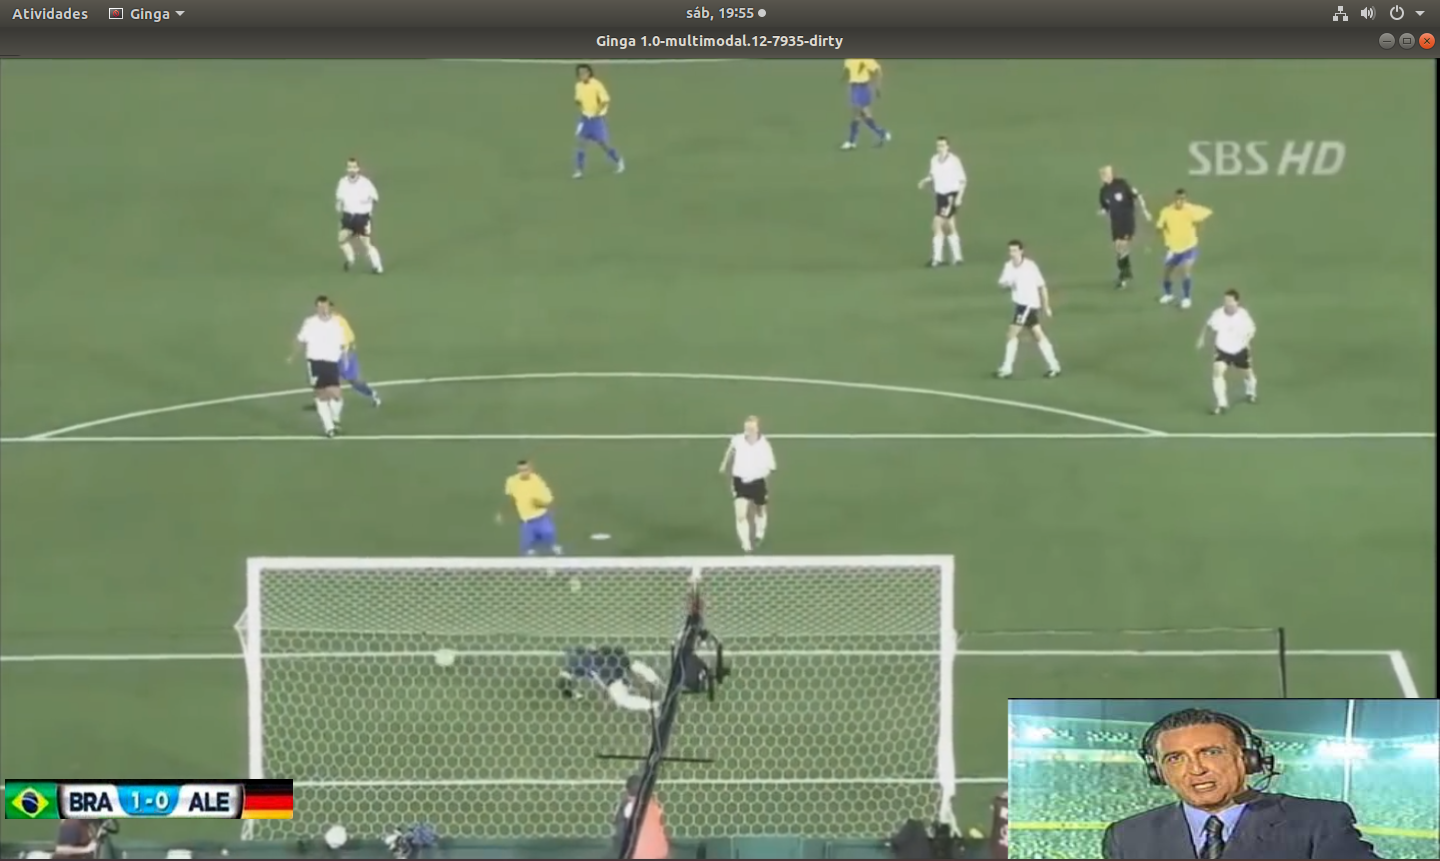
\includegraphics[width=1\textwidth]{figuras/Jogo1.png}
	   \vspace{-2.5cm}
	\end{minipage}
  } \hfill 	
  \subfloat[Depois que o usuário disser "put that"]
  {
    \label{fig:putThat2}
	\begin{minipage}[c][1\width]{0.48\textwidth}
	   \centering
	   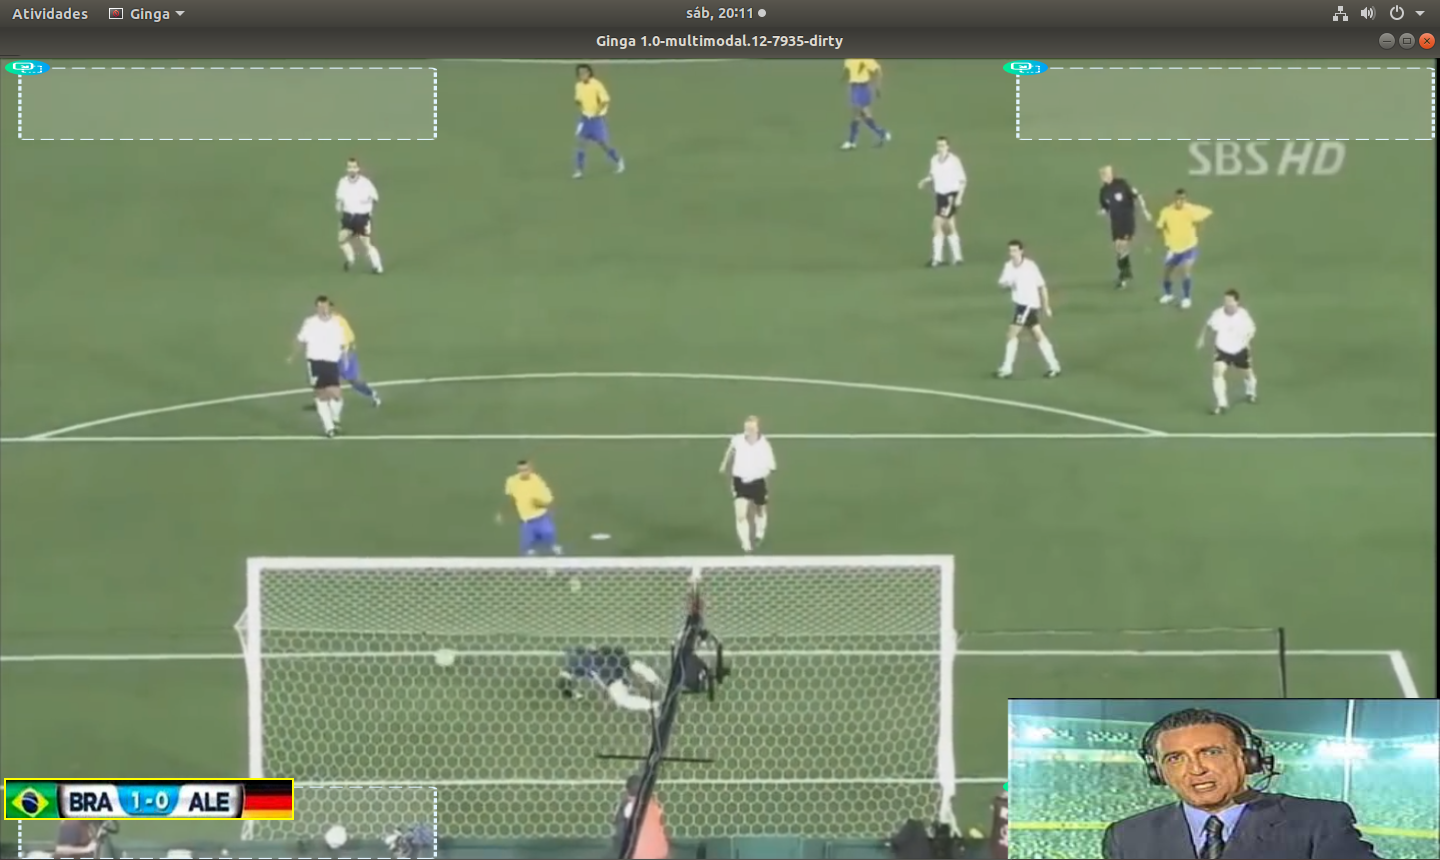
\includegraphics[width=1\textwidth]{figuras/Jogo2.png}
	   \vspace{-2.5cm}
	\end{minipage}
  }
  \vspace{-2cm}
  \newpage
  \subfloat[Depois que o usuário seleciona o ponto esquerdo]
  {
    \label{fig:putThat3}
	\begin{minipage}[c][1\width]{0.48\textwidth}
	   \centering
	   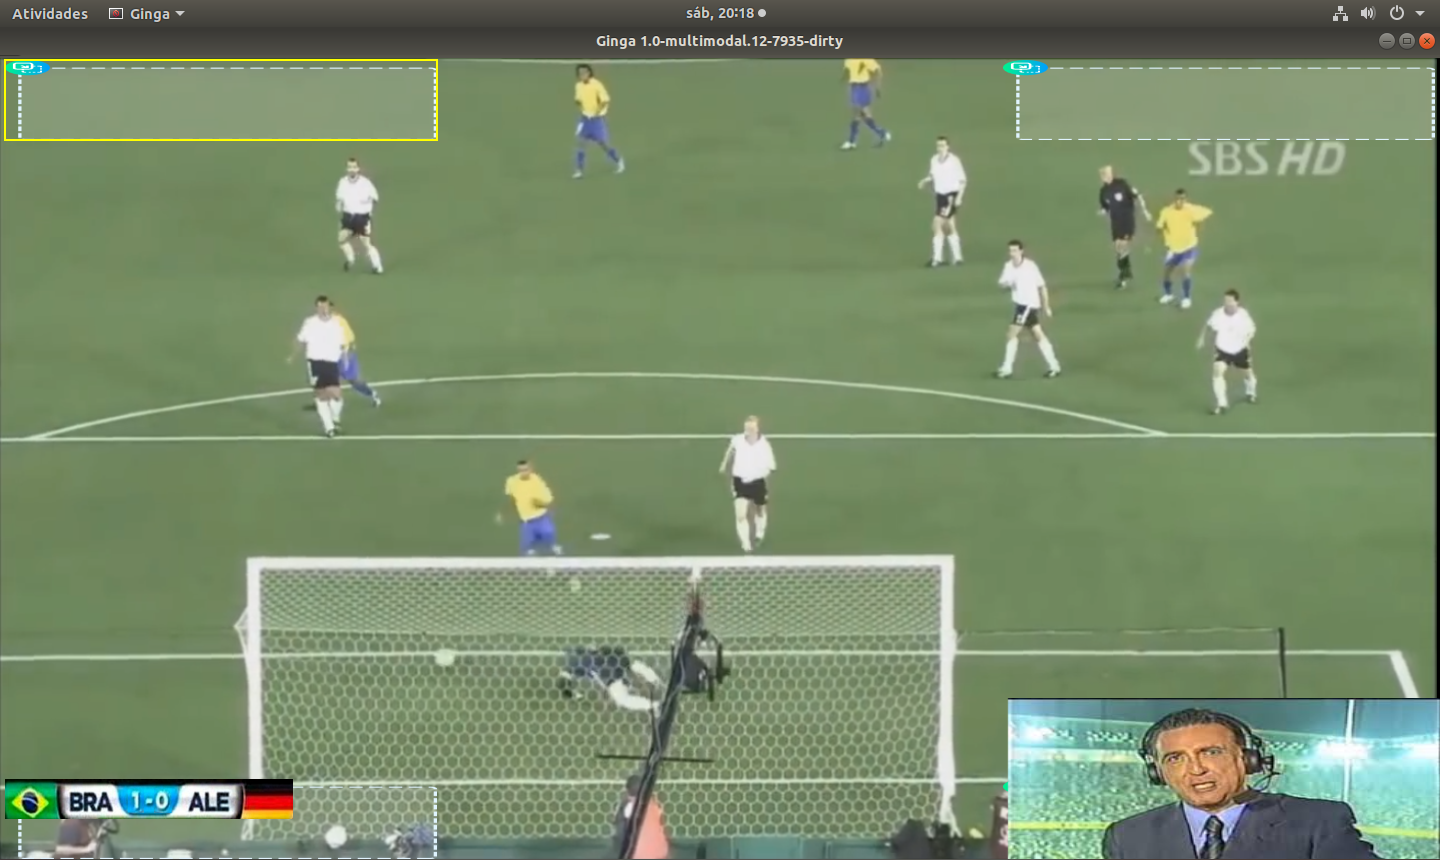
\includegraphics[width=1\textwidth]{figuras/Jogo3.png}
	   \vspace{-2.5cm}
	\end{minipage}
   } \hfill 	
   \subfloat[Depois que o usuários disser "there"]
   {
	\label{fig:putThat4}
	\begin{minipage}[c][1\width]{0.48\textwidth}
	   \centering
	   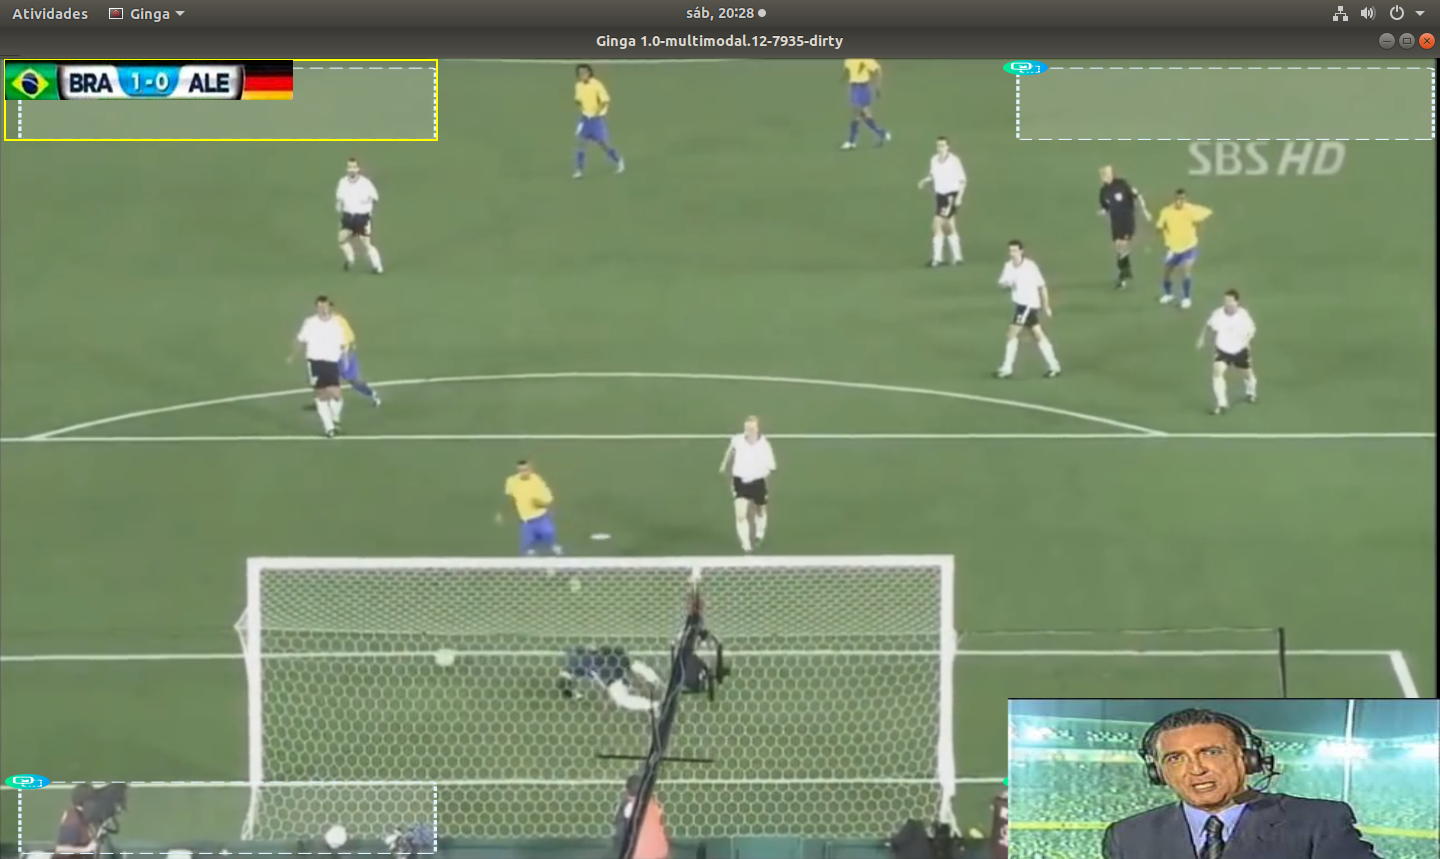
\includegraphics[width=1\textwidth]{figuras/Jogo4.png}
	   \vspace{-2.5cm}
	\end{minipage}
   }
	\vspace{-2cm}
	\newpage
	\begin{center}
	\subfloat[Depois que a interação terminar]
	{
	  \label{fig:putThat5}
	  \begin{minipage}[c][1\width]{
	   0.6\textwidth}
	   \centering
	   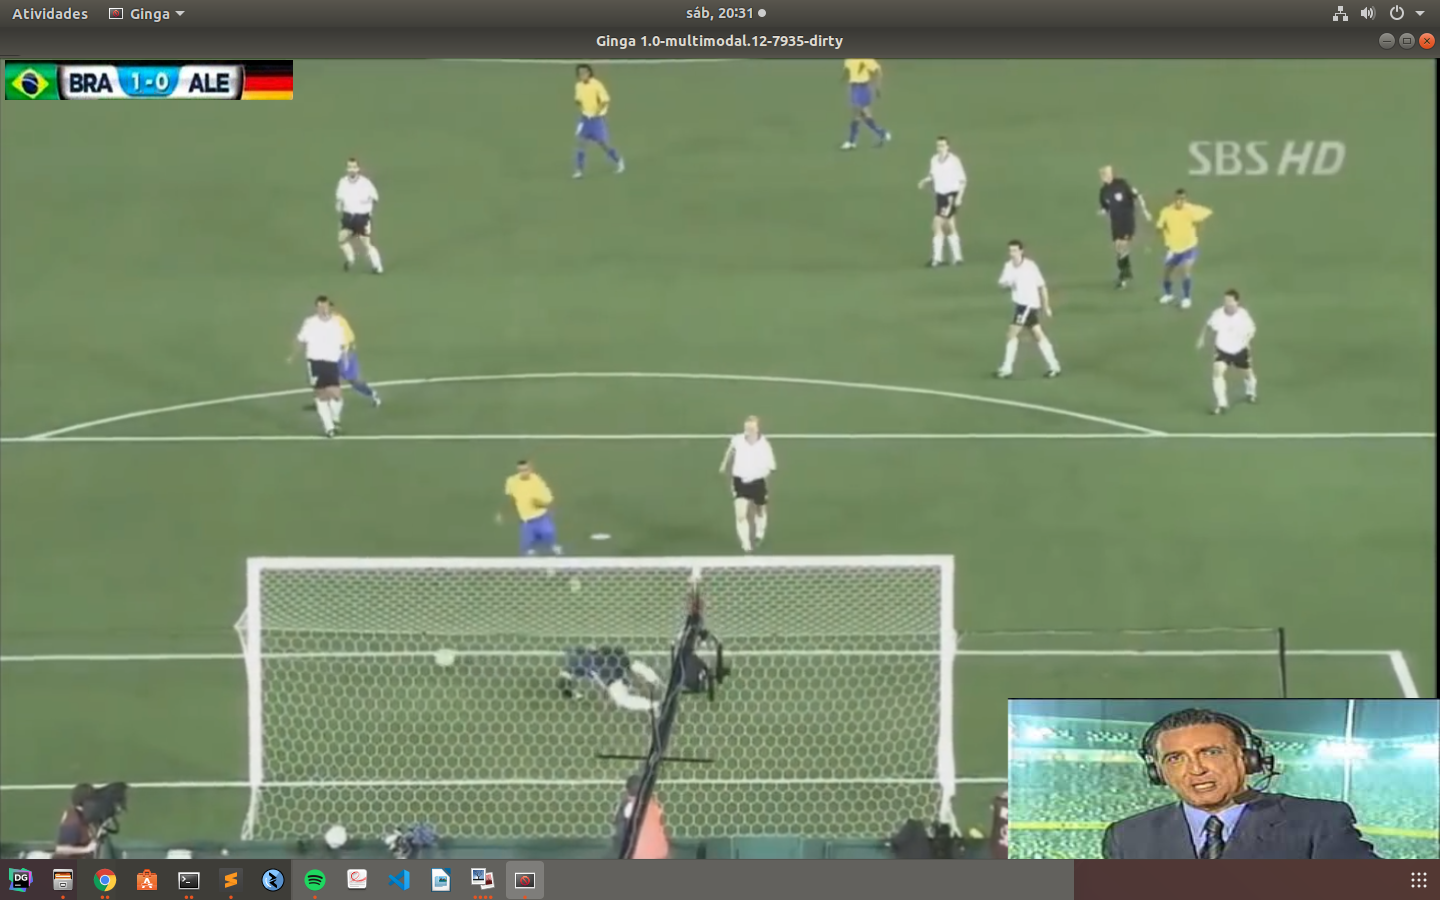
\includegraphics[width=1\textwidth]{figuras/Jogo5.png}
	   \vspace{-2.5cm}
	  \end{minipage}
	}
	\end{center}
\caption{Instantes do aplicativo em execução após cada interação do usuário}
\end{figure}


\section{Multiusuário} \label{sec:casoUsoMultiusuario}

Nesta seção apresenta casos de uso onde a participação e identificação do usuário representa uma interessante funcionalidade tendo em vista a importância da participação da TV Digital na vida das pessoas.  

\subsection{Limitação de interação} \label{sec:casoUsoLimiteInteracao}
Neste caso de uso, somente os usuários \textit{U01} e \textit{U02} atendem o perfil. Suas propriedades, incluindo o \textit{id}, estão armazenadas nos arquivos \textit{usr1.xml} e \textit{usr2.xml} respectivamente. A aplicação é apresentada na Listagem~\ref{lst:appIdMultUser}.

\begin{lstlisting}[language=ncl,label=lst:appIdMultUser, caption={Código da aplicação NCL com identificação multiusuário.}]
<?xml version="1.0" encoding="ISO-8859-1"?>
<ncl id="aplNCL40MultUser" xmlns="http://www.ncl.org.br/NCL4.0/EDTVProfile">
 <head>
	<regionBase>
		<region id="florestaVideoReg" width="100%" height="100%" zIndex="0" />
	</regionBase>
	<descriptorBase>
	    <descriptor id="florestaVideoRegDesc"  region="florestaVideoReg" />
	</descriptorBase>
	<connectorBase>
       <causalConnector id="onVoiceRecognitionPause">
          <connectorParam name="key"/>
          <connectorParam name="user"/>      
          <simpleCondition role="onVoiceRecognition" key="$\$$key" user="$\$$user"/>
          <simpleAction role="pause" />
       </causalConnector>  
       <causalConnector id="onVoiceRecognitionResume">
          <connectorParam name="key"/>
          <connectorParam name="user"/>      
          <simpleCondition role="onVoiceRecognition" key="$\$$key" user="$\$$user"/>
          <simpleAction role="resume" />
       </causalConnector>  
       <causalConnector id="onVoiceRecognitionStop">
          <connectorParam name="key"/>
          <connectorParam name="user"/>      
          <simpleCondition role="onVoiceRecognition" key="$\$$key" user="$\$$user"/>
          <simpleAction role="stop" />
       </causalConnector>  
	</connectorBase>
    <userBase>
      <userProfile id="profile1" src="profiles/profile.xml"/>
    </userBase>
  </head>
<body>
	<port id="pVideo" component="florestaVideo" />
	<media id="florestaVideo" src="videos/forest_720.mp4" descriptor="florestaVideoRegDesc"/>
    <link xconnector="onVoiceRecognitionPause">
          <bind role="onVoiceRecognition" component="florestaVideo">
            <bindParam name="key" value="pausar"/>
            <bindParam name="user" value="profile1"/>
          </bind>
          <bind role="pause" component="florestaVideo"/>
    </link> 
    <link xconnector="onVoiceRecognitionResume">
          <bind role="onVoiceRecognition" component="florestaVideo">
            <bindParam name="key" value="tocar"/>
            <bindParam name="user" value="profile1"/>            
          </bind>
          <bind role="resume" component="florestaVideo"/>
    </link> 
    <link xconnector="onVoiceRecognitionStop">
          <bind role="onVoiceRecognition" component="florestaVideo">
            <bindParam name="key" value="parar"/>
            <bindParam name="user" value="profile1"/>            
          </bind>
          <bind role="stop" component="florestaVideo"/>
    </link> 
 </body>
</ncl>
\end{lstlisting}

\subsection{Identificação do usuário} \label{sec:casoUsoIdentificaçãoInteracao}

A aplicação desenvolvida possui uma mídia que será executada com o início do documento NCL. O conteúdo do vídeo apresenta uma floresta com neve e em um determinado momento será apresentada uma imagem vendendo um passeio de esqui. No momento que o usuário diz ``comprar'', a aplicação vai informar quem comprou o passeio identificando a interação. Porém, aplicação só irá responder se a interação vier de um dos usuários que atendem o perfil definido no profile. A aplicação é apresentada na Listagem~\ref{lst:appIntMultUser}.

\begin{figure}[h!] 
    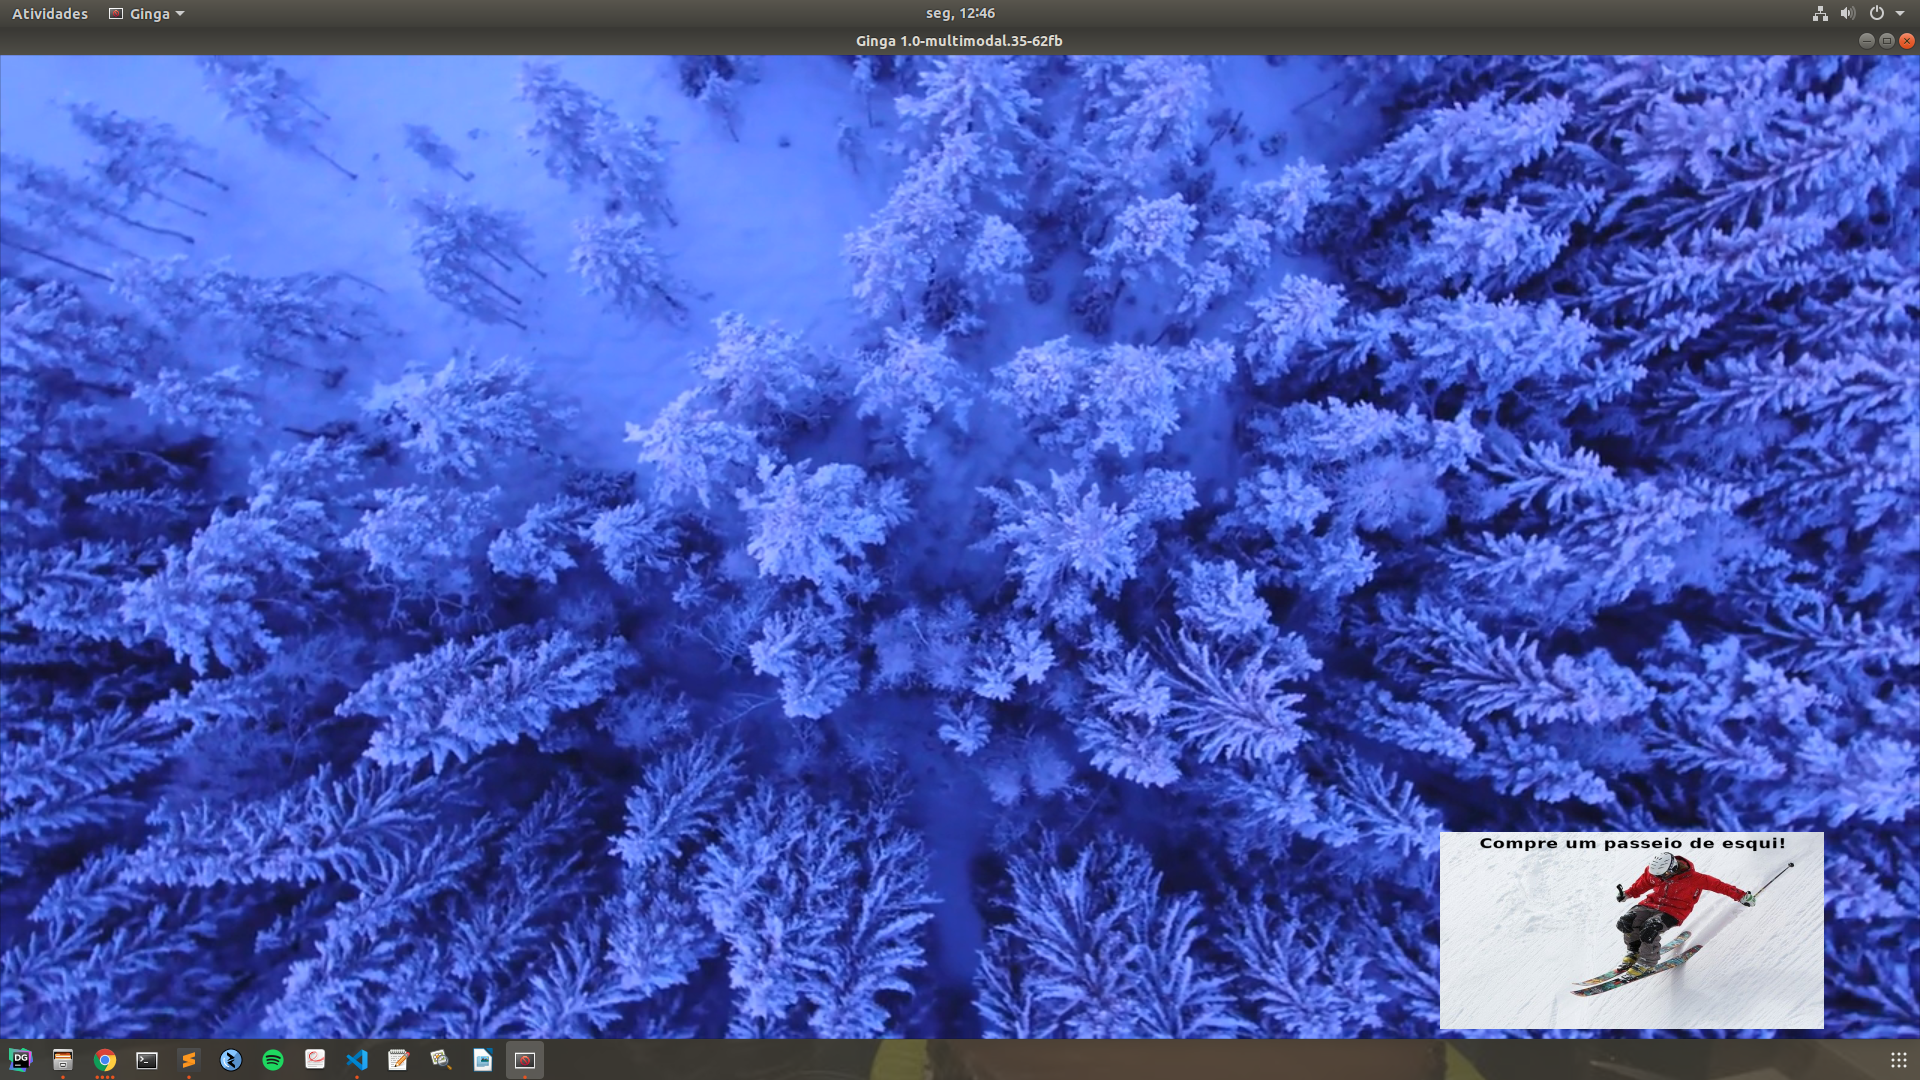
\includegraphics[scale=0.2]{figuras/appMultUser.png}
    \centering
    \caption{Interface da aplicação com interação multiuser.}
    \label{fig:appMultUser}
\end{figure}
\vspace{-0.2cm}

\begin{lstlisting}[language=ncl,label=lst:appIntMultUser, caption={Código da aplicação NCL com interação multiusuário.}]
<?xml version="1.0" encoding="ISO-8859-1"?>
<ncl id="aplMultiUser" xmlns="http://www.ncl.org.br/NCL3.0/EDTVProfile">
<head>
  <regionBase>
    <region id="VideoReg" width="100%" height="100%" zIndex="0" />
    <region id="ImgPropagandaReg" right="5%" bottom="5%" width="20%" height="20%" zIndex="2"/>  
    <region id="rg1" left="5%" bottom="5%" height="10%"  width="50%" />
  </regionBase>
  <descriptorBase>
      <descriptor id="VideoDesc"  region="VideoReg"/>  
      <descriptor id="ImgPropagandaDesc"  region="ImgPropagandaReg"  />
      <descriptor id="desc1"  region="rg1"/> 
  </descriptorBase>
  <userBase>
      <userProfile id="profile1" src="profiles/profile.xml"/>
  </userBase>
  <connectorBase>
      <causalConnector id="onBeginStart">
        <simpleCondition role="onBegin"/>
        <simpleAction role="start" max="unbounded"/>
      </causalConnector> 
      <causalConnector id="onVoiceRecognitionSet">
        <connectorParam name="key"/>
        <connectorParam name="user"/>      
        <connectorParam name="var"/>      
        <simpleCondition role="onVoiceRecognition" key="$\$$key" user="$\$$user"/>
        <simpleAction role="set" value="$\$$var"/>
      </causalConnector>
  </connectorBase>
</head>
<body>
    <port id="pInicio" component="lua" />
    <port id="pVideo" component="snowVideo"/>
    <media id="lua" src="scripts/script.lua" type= "application/x-ginga-NCLua" descriptor="desc1">
      <property name="usr" value="false"/>
    </media>
    <media id="ImgPropaganda" src="images/passeioEsqui.jpeg" descriptor="ImgPropagandaDesc">
      <property name="usr" value="false"/>
    </media>
    <media id="snowVideo" src="videos/snow_720.mp4" descriptor="VideoDesc">
      <property name="usr" value="false"/>
      <area id="aPropaganda" begin="2s" /> 
    </media>
    <link xconnector="onBeginStart">
        <bind role="onBegin" component="snowVideo" interface="aPropaganda"/>
        <bind role="start" component="ImgPropaganda"/>
    </link>
    <link xconnector="onVoiceRecognitionSet">
      <bind role="onVoiceRecognition" component="ImgPropaganda">
          <bindParam name="key" value="comprar"/>
          <bindParam name="user" value="profile1"/>
      </bind> 
      <bind role="getValue" component="ImgPropaganda" interface="usr"/>
        <bind role="set" component="lua" interface="usr">
            <bindParam name="var" value="$\$$getValue"/>
        </bind>
    </link>
</body>
</ncl>
\end{lstlisting}

No próximo capitulo será abordado as considerações finais desta tese contendo conclusões e trabalhos futuros.




% --- -----------------------------------------------------------------
% --- Referencias Bibliograficas. (Obrigatorio)
% --- -----------------------------------------------------------------
\cleardoublepage
\bibliographystyle{acm-2} % abbrv - abnt-num
%\bibliographystyle{uff-ic}
\bibliography{bibliografia} % arquivo fonte com a bibilografia

% --- -----------------------------------------------------------------
% --- Apendice.(Opcional)
% --- -----------------------------------------------------------------
%\cleardoublepage
%\appendix
%\chapter{<T\'ITULO DO AP\^ENDICE>}
\label{apend}

% Este apêndice apresenta informações complementares.

Elemento opcional. O(s) apêndice(s) são identificados por letras maiúsculas consecutivas, travessão e pelos respectivos títulos. Excepcionalmente utilizam-se letras maiúsculas dobradas, na identificação, quando esgotadas as 23 letras do alfabeto (ABNT, 2005).


\end{document}